\chapter{信息几何}
\label{chap:information-geometry}

在高斯族$\mathcal{N}(\mu,\sigma^{2})$中把均值增加$0.5$。若$\sigma=0.5$，新旧两个密度的峰几乎错开，两者的KL散度等于$0.5$；若$\sigma=2$，两条钟形曲线几乎重合，KL散度只有$1/32$。参数走了同样远，分布却变化了相差十六倍的量，如图~\ref{fig:igeo-same-shift}。

\begin{BookInlineFigure}
  \centering
  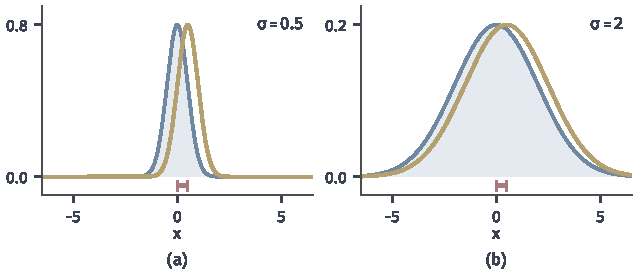
\includegraphics[width=108mm]{figures/07-probability/07-distribution-optimization/matplotlib/igeo-same-shift/figure.pdf}
  \caption{同样的均值位移$0.5$（红色短线）在两个尺度下引起的变化。蓝线并加浅蓝底是$\mathcal{N}(0,\sigma^{2})$，黄线是$\mathcal{N}(0.5,\sigma^{2})$。(a)$\sigma=0.5$，两者的KL散度为$0.5$；(b)$\sigma=2$，KL散度为$1/32$。}
  \label{fig:igeo-same-shift}
\end{BookInlineFigure}

方差方向也一样。把方差从$0.1$增加到$0.2$，KL散度约为$0.097$；把方差从$10$增加到$10.1$，KL散度只有约$2.5\times10^{-5}$。若改用对数方差$\tau=\ln\sigma^{2}$作参数，情况又不同：$\tau$增加同一个量，KL散度与起点的方差无关。参数的欧氏长度不是分布变化的尺度，而且换一套坐标，数值关系就跟着改变。

第~\ref{chap:distribution-approximation}章把族内逼近写成有限维参数的优化。普通梯度下降默认参数的每个方向“一样贵”，上面的例子说明这一默认并不成立：在$\sigma$很小的地方，均值稍动一点分布就大变；在方差很大的地方，方差改动很多分布也几乎不变。本章研究三个问题：参数的微小位移怎样引起分布变化，这种变化的大小用什么来度量；换一套参数坐标时，这个度量中什么改变、什么不变；怎样用它选择参数的更新方向。把分布族当作带有这种局部尺度的几何对象来研究，这套方法称为\term{信息几何}（information geometry）。

第一节规定可以逐点求导、并能与积分交换的分布族，定义得分函数与Fisher信息。第二节由邻近分布之间KL散度的二阶展开说明Fisher信息正是局部尺度，再检查它在坐标变换下的规律。第三节在指数族中核验这些结构，对数配分函数的导数同时给出Fisher信息与两套坐标的转换。第四节在相同的局部分布变化下寻找目标下降最多的方向，得到自然梯度，并说明它与坐标的关系。第五节讨论怎样实际计算这个方向和步长。

本章用到第~\ref{chap:distribution-families}章的指数族与均值映射，第~\ref{chap:distribution-comparison}章的KL散度及两个高斯分布之间的KL公式，以及第~\ref{chap:distribution-approximation}章的逼近目标。全章贯穿高斯族$\mathcal{N}(\mu,\sigma^{2})$在几套坐标下的计算。

\section{正则分布族}
\label{sec:igeo-regular}

要谈“参数动一点，分布变多少”，先得让“动一点”在每个位置上都有意义。固定可测空间$(\mathcal{X},\mathcal{F})$上的一个$\sigma$有限参考测度$\nu$，参数$\bm{\theta}$取值于$\mathbb{R}^{k}$的子集$\Theta$，每个$\bm{\theta}$对应一个相对$\nu$的密度$p_{\bm{\theta}}$与概率分布$P_{\bm{\theta}}$。对固定的$x$，$p_{\bm{\theta}}(x)$是$\bm{\theta}$的普通函数，可以对它求偏导数；分布的变化却还要把这些逐点的变化积分起来。于是需要两类条件：逐点可微，以及求导与积分可以交换。

\begin{definition}[正则分布族]
\label{def:igeo-regular-family}
称$\{p_{\bm{\theta}}:\bm{\theta}\in\Theta\}$为\term{正则分布族}（regular family），若下列条件成立：
\begin{enumerate}
  \item $\Theta$是$\mathbb{R}^{k}$中的非空开集；
  \item 支撑$S=\{x:p_{\bm{\theta}}(x)>0\}$不依赖$\bm{\theta}$；
  \item 对每个$x\in S$，$\bm{\theta}\mapsto p_{\bm{\theta}}(x)$在$\Theta$上连续可微；
  \item 对每个$\bm{\theta}\in\Theta$，$\int_{S}\lVert\nabla_{\bm{\theta}}p_{\bm{\theta}}\rVert_2\,\mathrm{d}\nu<\infty$，并且
  \begin{equation}
    \int_{S}\nabla_{\bm{\theta}}p_{\bm{\theta}}(x)\,\nu(\mathrm{d}x)=\nabla_{\bm{\theta}}\int_{S}p_{\bm{\theta}}(x)\,\nu(\mathrm{d}x)=\bm{0}.
    \label{eq:igeo-exchange}
  \end{equation}
\end{enumerate}
\end{definition}

四个条件各管一件事。开集保证从$\bm{\theta}$出发可以朝任何方向走一小步而不离开参数范围。共同支撑保证$\ln p_{\bm{\theta}}(x)$对所有参数都在同一个集合$S$上有定义，比较两个邻近分布时不会出现一边有质量、另一边为零的位置。逐点可微给出每个位置上密度的变化率。最后一条说：先对每个位置求变化率再积分，等于先积分再求导；而积分恒为$1$，所以结果为零向量。

式~\eqref{eq:igeo-exchange}的交换通常用控制收敛来保证。设$\bm{\theta}$有一个凸邻域$U$和$\nu$可积的函数$M$，使对所有$\bm{\theta}'\in U$与$x\in S$有
\[
  \lVert\nabla_{\bm{\theta}}p_{\bm{\theta}'}(x)\rVert_2\leq M(x).
\]
由中值定理，沿任一坐标方向的差商$\bigl(p_{\bm{\theta}+h\bm{e}_j}(x)-p_{\bm{\theta}}(x)\bigr)/h$的绝对值不超过$M(x)$，而当$h\to0$时它逐点趋于偏导数；控制收敛定理于是允许在积分号下取这个极限，可参考\BookChapterRef{chap:integration}{卷四第6章“积分”}。高斯族就满足这一条件：参数限制在紧邻域内时，密度的偏导数不超过一个多项式乘以$\mathrm{e}^{-cx^{2}}$，后者可积。

定义里没有要求后面将定义的Fisher信息正定。正则性只保证一阶的计算可以进行；参数是否冗余、局部变化是否退化，是另外需要检查的事情。

\subsection{得分函数}
\label{sec:igeo-score}

参数从$\bm{\theta}$变到$\bm{\theta}+\bm{\delta}$时，位置$x$处的密度从$p_{\bm{\theta}}(x)$变到$p_{\bm{\theta}+\bm{\delta}}(x)$。比较两个分布时，要紧的往往不是密度差了多少，而是差了百分之几：KL散度、似然比都只依赖密度之比。一阶近似下，相对变化是
\[
  \frac{p_{\bm{\theta}+\bm{\delta}}(x)-p_{\bm{\theta}}(x)}{p_{\bm{\theta}}(x)}\approx\frac{\langle\nabla_{\bm{\theta}}p_{\bm{\theta}}(x),\bm{\delta}\rangle}{p_{\bm{\theta}}(x)}=\langle\nabla_{\bm{\theta}}\ln p_{\bm{\theta}}(x),\bm{\delta}\rangle .
\]
尾部某个位置的密度可能很小，绝对变化也很小，但相对变化可以很大；对数导数正好记录的是后者。

\begin{definition}[得分函数]
\label{def:igeo-score}
设分布族正则。对$x\in S$，称
\begin{equation}
  \bm{s}_{\bm{\theta}}(x)=\nabla_{\bm{\theta}}\ln p_{\bm{\theta}}(x)=\frac{\nabla_{\bm{\theta}}p_{\bm{\theta}}(x)}{p_{\bm{\theta}}(x)}
  \label{eq:igeo-score}
\end{equation}
为\term{得分函数}（score function）。它是$\mathbb{R}^{k}$值函数，第$j$个分量记录沿第$j$个参数方向，$x$处密度的相对变化率。
\end{definition}

把概率看成总量为$1$的质量，参数变化只是把质量在各位置之间重新分配，不能凭空增减。某些位置的质量相对增加，另一些位置就必须相对减少，按质量加权以后正负抵消。下面的引理把这一点写成公式。

\begin{lemma}[得分的期望为零]
\label{lem:igeo-score-mean}
设分布族正则，$X\sim P_{\bm{\theta}}$，则$\mathbb{E}_{\bm{\theta}}\lVert\bm{s}_{\bm{\theta}}(X)\rVert_2<\infty$，并且
\begin{equation}
  \mathbb{E}_{\bm{\theta}}[\bm{s}_{\bm{\theta}}(X)]=\bm{0}.
  \label{eq:igeo-score-mean}
\end{equation}
\end{lemma}

\begin{proof}
$P_{\bm{\theta}}$的质量全部在$S$上；在$S$上，由式~\eqref{eq:igeo-score}，得分乘以密度就是密度的梯度。于是
\[
  \mathbb{E}_{\bm{\theta}}\lVert\bm{s}_{\bm{\theta}}(X)\rVert_2=\int_{S}\frac{\lVert\nabla_{\bm{\theta}}p_{\bm{\theta}}\rVert_2}{p_{\bm{\theta}}}\,p_{\bm{\theta}}\,\mathrm{d}\nu=\int_{S}\lVert\nabla_{\bm{\theta}}p_{\bm{\theta}}\rVert_2\,\mathrm{d}\nu<\infty ,
\]
期望存在。同样地，
\[
  \mathbb{E}_{\bm{\theta}}[\bm{s}_{\bm{\theta}}(X)]=\int_{S}\nabla_{\bm{\theta}}p_{\bm{\theta}}\,\mathrm{d}\nu ,
\]
由式~\eqref{eq:igeo-exchange}，右端为零向量。
\end{proof}

\paragraph{高斯族的两个得分}
取$\nu$为Lebesgue测度，参数为$(\mu,\sigma)$，$\sigma>0$。对数密度是
\[
  \ln p_{\mu,\sigma}(x)=-\ln\sigma-\frac12\ln(2\pi)-\frac{(x-\mu)^{2}}{2\sigma^{2}} .
\]
记标准化的位置$z=(x-\mu)/\sigma$。分别对$\mu$与$\sigma$求偏导数，得到
\begin{equation}
  s_{\mu}(x)=\frac{x-\mu}{\sigma^{2}}=\frac{z}{\sigma},\qquad
  s_{\sigma}(x)=-\frac1\sigma+\frac{(x-\mu)^{2}}{\sigma^{3}}=\frac{z^{2}-1}{\sigma}.
  \label{eq:igeo-gauss-score}
\end{equation}
$Z=(X-\mu)/\sigma$服从$\mathcal{N}(0,1)$，$\mathbb{E}[Z]=0$，$\mathbb{E}[Z^{2}]=1$，所以两个得分的期望都是零，与引理~\ref{lem:igeo-score-mean}一致。

两个得分讲的是两种不同的重新分配。增大均值时，$s_{\mu}$在$x>\mu$处为正、在$x<\mu$处为负：右边的质量相对增加，左边相对减少，整体向右挪。增大$\sigma$时，$s_{\sigma}$在$\lvert z\rvert>1$处为正、在$\lvert z\rvert<1$处为负：中间的质量被搬到两边的尾部。图~\ref{fig:igeo-score-density}的下排画出$p\,s=\partial p/\partial\theta$，浅蓝与浅红两块面积相等，这正是式~\eqref{eq:igeo-score-mean}。

\begin{BookInlineFigure}
  \centering
  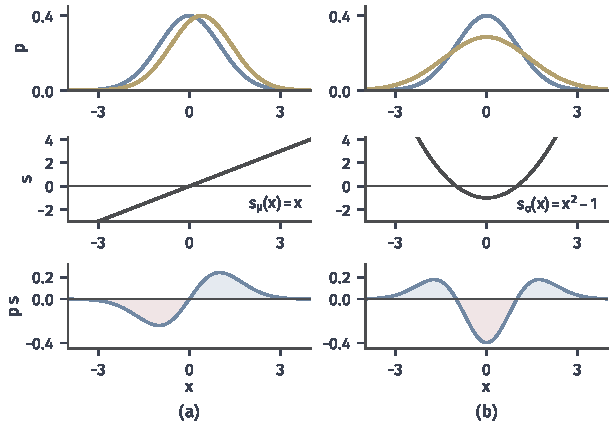
\includegraphics[width=104mm]{figures/07-probability/07-distribution-optimization/matplotlib/igeo-score-density/figure.pdf}
  \caption{$\mathcal{N}(0,1)$处的两个得分。(a)改变均值；(b)改变尺度$\sigma$。上排：蓝线为$\mathcal{N}(0,1)$，黄线为参数改变后的密度（(a)为$\mathcal{N}(0.4,1)$，(b)为$\mathcal{N}(0,1.4^{2})$）。中排：得分函数$s(x)$。下排：密度对参数的导数$p\,s$，浅蓝为质量相对增加的区域，浅红为相对减少的区域，两块面积相等，(a)中各约$0.399$，(b)中各约$0.483$。}
  \label{fig:igeo-score-density}
\end{BookInlineFigure}

\paragraph{支撑随参数移动}
共同支撑不能省。取$\operatorname{Unif}(0,\theta)$，$\theta>0$，在$(0,\theta)$上$p_{\theta}(x)=1/\theta$。对这些$x$，
\[
  \frac{\partial}{\partial\theta}\ln p_{\theta}(x)=-\frac1\theta ,
\]
它是常数，期望等于$-1/\theta\neq0$。引理~\ref{lem:igeo-score-mean}失效，原因是对积分上限也随$\theta$变化的积分求导会多出一项边界值：
\[
  \frac{\mathrm{d}}{\mathrm{d}\theta}\int_{0}^{\theta}\frac1\theta\,\mathrm{d}x=\underbrace{\frac1\theta}_{\text{边界项}}+\int_{0}^{\theta}\Bigl(-\frac1{\theta^{2}}\Bigr)\mathrm{d}x=\frac1\theta-\frac1\theta=0 .
\]
积分号内的部分正是得分的期望$-1/\theta$；边界项$1/\theta$是新出现在$\theta$右侧的质量，得分只定义在旧支撑上，看不到它。

图~\ref{fig:igeo-uniform-boundary}把这一点画了出来。$\theta$增大到$\theta+h$时，旧支撑内的密度整体下降，损失的质量$h/(\theta+h)$恰好出现在旧支撑外的$(\theta,\theta+h]$上。质量守恒的类比在这里仍然成立，只是新增的那部分落在得分看不到的地方。对这类模型，后面关于Fisher信息与局部KL的结论都不能直接套用：只要$h<0$，$P_{\theta}$在$(\theta+h,\theta)$上有质量而$P_{\theta+h}$没有，于是
\[
  D_{\mathrm{KL}}(P_{\theta}\Vert P_{\theta+h})=\infty .
\]

\begin{BookInlineFigure}
  \centering
  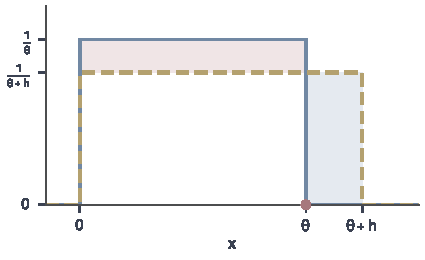
\includegraphics[width=72mm]{figures/07-probability/07-distribution-optimization/matplotlib/igeo-uniform-boundary/figure.pdf}
  \caption{支撑随参数移动的均匀分布，$\theta=1$，$h=0.25$。蓝线为$\operatorname{Unif}(0,\theta)$的密度，黄色虚线为$\operatorname{Unif}(0,\theta+h)$的密度。浅红区域是旧支撑内减少的质量$0.2$，浅蓝区域是旧支撑外新增的质量$0.2$；红点标出移动的端点。}
  \label{fig:igeo-uniform-boundary}
\end{BookInlineFigure}

\subsection{Fisher信息}
\label{sec:igeo-fisher}

得分是一个均值为零的随机向量。它的取值越分散，参数的小变化在各处造成的相对变化就越大，分布也就越容易与原来区分开。沿方向$\bm{u}\in\mathbb{R}^{k}$，密度的相对变化率是$\langle\bm{u},\bm{s}_{\bm{\theta}}(X)\rangle$，它的均方
\[
  \mathbb{E}_{\bm{\theta}}\bigl[\langle\bm{u},\bm{s}_{\bm{\theta}}(X)\rangle^{2}\bigr]=\bm{u}^{\top}\,\mathbb{E}_{\bm{\theta}}\bigl[\bm{s}_{\bm{\theta}}(X)\bm{s}_{\bm{\theta}}(X)^{\top}\bigr]\,\bm{u}
\]
是一个关于$\bm{u}$的二次型。中间的矩阵把所有方向的信息收在一起。

\begin{definition}[Fisher信息矩阵]
\label{def:igeo-fisher}
设分布族正则，且$\mathbb{E}_{\bm{\theta}}\lVert\bm{s}_{\bm{\theta}}(X)\rVert_2^{2}<\infty$。称$k\times k$矩阵
\begin{equation}
  \bm{G}(\bm{\theta})=\mathbb{E}_{\bm{\theta}}\bigl[\bm{s}_{\bm{\theta}}(X)\bm{s}_{\bm{\theta}}(X)^{\top}\bigr]
  \label{eq:igeo-fisher}
\end{equation}
为$\bm{\theta}$处的\term{Fisher信息矩阵}（Fisher information matrix），简称Fisher信息。
\end{definition}

由引理~\ref{lem:igeo-score-mean}，得分的均值为零，所以
\[
  \bm{G}(\bm{\theta})=\operatorname{Cov}_{\bm{\theta}}\bigl(\bm{s}_{\bm{\theta}}(X)\bigr),
\]
Fisher信息就是得分的协方差矩阵。这里用$\bm{G}$而不用常见的$I$，是为了与互信息$I(X;Y)$区分。

Fisher信息总是对称半正定的。对任意$\bm{u}$，
\[
  \bm{u}^{\top}\bm{G}(\bm{\theta})\bm{u}=\mathbb{E}_{\bm{\theta}}\bigl[\langle\bm{u},\bm{s}_{\bm{\theta}}(X)\rangle^{2}\bigr]\geq0 .
\]
等号成立当且仅当$\langle\bm{u},\bm{s}_{\bm{\theta}}(X)\rangle=0$几乎必然成立，也就是沿$\bm{u}$方向，几乎每个位置上密度的一阶变化率都是零。这样的方向在一阶意义下不改变分布。$\bm{G}$是否正定，取决于有没有这样的方向，正则性并不排除它们。

\paragraph{高斯族的信息矩阵}
由式~\eqref{eq:igeo-gauss-score}，三个乘积的期望要用到标准正态的矩$\mathbb{E}[Z^{2}]=1$、$\mathbb{E}[Z^{3}]=0$、$\mathbb{E}[Z^{4}]=3$。逐项计算：
\[
  \mathbb{E}[s_{\mu}^{2}]=\frac{\mathbb{E}[Z^{2}]}{\sigma^{2}}=\frac{1}{\sigma^{2}},\qquad
  \mathbb{E}[s_{\mu}s_{\sigma}]=\frac{\mathbb{E}[Z^{3}]-\mathbb{E}[Z]}{\sigma^{2}}=0,
\]
\[
  \mathbb{E}[s_{\sigma}^{2}]=\frac{\mathbb{E}[Z^{4}]-2\mathbb{E}[Z^{2}]+1}{\sigma^{2}}=\frac{3-2+1}{\sigma^{2}}=\frac{2}{\sigma^{2}} .
\]
于是在坐标$(\mu,\sigma)$下
\begin{equation}
  \bm{G}(\mu,\sigma)=\begin{bmatrix}1/\sigma^{2}&0\\0&2/\sigma^{2}\end{bmatrix}.
  \label{eq:igeo-gauss-fisher}
\end{equation}
两个对角元都与$1/\sigma^{2}$成正比：分布越窄，同样的参数改动越容易被察觉。这正是章首例子中$\sigma=0.5$与$\sigma=2$相差$16=(2/0.5)^{2}$倍的来源，下一节会把这一关系写成一般的结论。非对角元为零，表示在这套坐标下，平移与伸缩引起的相对变化不相关。

\paragraph{退化的信息}
Fisher信息为零或奇异，可能出于几种不同的原因，需要分开辨认。看三个只有均值变化的单位方差高斯族：
\[
  \mathcal{N}(\theta^{3},1),\qquad\mathcal{N}(\theta^{2},1),\qquad\mathcal{N}(a+b,1).
\]
若均值是参数的可微函数$m(\bm{\theta})$，链式法则给出得分$(x-m(\bm{\theta}))\nabla m(\bm{\theta})$，再由$\mathbb{E}[(X-m)^{2}]=1$得到
\[
  \bm{G}(\bm{\theta})=\nabla m(\bm{\theta})\,\nabla m(\bm{\theta})^{\top}.
\]

第一个族$\mathcal{N}(\theta^{3},1)$：$G(\theta)=9\theta^{4}$，在$\theta=0$处为零。但$\theta\mapsto\theta^{3}$是单射，不同的$\theta$给出不同的分布，参数是可辨识的。$\theta=0$处退化只说明一阶变化消失：由第~\ref{chap:distribution-comparison}章等方差高斯分布的KL公式，
\[
  D_{\mathrm{KL}}\bigl(\mathcal{N}(0,1)\Vert\mathcal{N}(\delta^{3},1)\bigr)=\frac{\delta^{6}}{2}>0,
\]
分布确实在变，只是变化从六阶才开始。

第二个族$\mathcal{N}(\theta^{2},1)$：$G(\theta)=4\theta^{2}$，在$\theta\neq0$处为正，局部看每一点附近的分布互不相同；但$\theta$与$-\theta$给出同一个分布，参数在整体上不可辨识。第三个族$\mathcal{N}(a+b,1)$：
\[
  \bm{G}(a,b)=\begin{bmatrix}1&1\\1&1\end{bmatrix},
\]
处处奇异，零空间沿$(1,-1)$方向。沿这个方向走，$a+b$不变，分布完全不变，这是参数冗余。

\begin{BookInlineFigure}
  \centering
  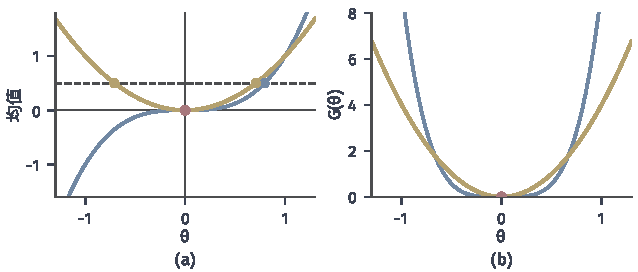
\includegraphics[width=108mm]{figures/07-probability/07-distribution-optimization/matplotlib/igeo-cubic-information/figure.pdf}
  \caption{两个单参数高斯族$\mathcal{N}(\theta^{3},1)$（蓝）与$\mathcal{N}(\theta^{2},1)$（黄）。(a)均值随$\theta$的变化，深灰虚线为均值$0.5$，与蓝线交于一点、与黄线交于两点；(b)Fisher信息$9\theta^{4}$与$4\theta^{2}$。红点$\theta=0$处两者的信息都为零。}
  \label{fig:igeo-cubic-information}
\end{BookInlineFigure}

图~\ref{fig:igeo-cubic-information}把前两个族放在一起。三件事由此分开：参数冗余是整条方向上分布都不变，信息在那个方向上处处为零；局部一阶退化是某一点上分布的一阶变化消失，分布本身仍可辨识；全局可辨识则要求不同参数给出不同分布，它与某点的信息是否为零没有蕴含关系。后面凡是要对$\bm{G}(\bm{\theta})$求逆，都要另加它正定的假设，并在不满足时先弄清是哪一种情形。


\section{分布变化的局部尺度}
\label{sec:igeo-local-scale}

Fisher信息是从得分的二阶矩定义的，它是否真的衡量了“分布变了多少”？章首的均值位移给出一个线索。由第~\ref{chap:distribution-comparison}章两个等方差高斯分布的KL公式，
\[
  D_{\mathrm{KL}}\bigl(\mathcal{N}(\mu,\sigma^{2})\Vert\mathcal{N}(\mu+\delta,\sigma^{2})\bigr)=\frac{\delta^{2}}{2\sigma^{2}}=\frac12\,G_{\mu\mu}\,\delta^{2},
\]
其中$G_{\mu\mu}=1/\sigma^{2}$是式~\eqref{eq:igeo-gauss-fisher}的第一个对角元。$\delta=0.5$时，$\sigma=0.5$与$\sigma=2$分别给出$0.5$与$1/32$，正是章首的两个数。这一节先证明在一般的正则族中，邻近分布间的KL散度在二阶意义下都是$\frac12\bm{\delta}^{\top}\bm{G}\bm{\delta}$；再换参数坐标，看矩阵怎样变，它所表示的局部变化又是否保持。

\subsection{KL的二阶展开}
\label{sec:igeo-kl-expansion}

展开$D_{\mathrm{KL}}(P_{\bm{\theta}}\Vert P_{\bm{\theta}+\bm{\delta}})$，就是对$\ln p_{\bm{\theta}+\bm{\delta}}(x)$在$\bm{\theta}$处作Taylor展开再取期望。一阶项的期望是得分的期望，为零；二阶项的期望涉及对数密度的Hessian矩阵。先把这个期望与Fisher信息联系起来。

\begin{lemma}[信息等式]
\label{lem:igeo-information-identity}
设分布族正则，对每个$x\in S$，$\bm{\theta}\mapsto p_{\bm{\theta}}(x)$二阶连续可微；在给定的$\bm{\theta}$处，$\int_{S}\lVert\nabla_{\bm{\theta}}^{2}p_{\bm{\theta}}\rVert\,\mathrm{d}\nu<\infty$，$\bm{G}(\bm{\theta})$有限，并且二阶导数也可以与积分交换：
\begin{equation}
  \int_{S}\nabla_{\bm{\theta}}^{2}p_{\bm{\theta}}\,\mathrm{d}\nu=\nabla_{\bm{\theta}}^{2}\int_{S}p_{\bm{\theta}}\,\mathrm{d}\nu=\bm{0}.
  \label{eq:igeo-second-exchange}
\end{equation}
则
\begin{equation}
  \mathbb{E}_{\bm{\theta}}\bigl[\nabla_{\bm{\theta}}^{2}\ln p_{\bm{\theta}}(X)\bigr]=-\bm{G}(\bm{\theta}).
  \label{eq:igeo-information-identity}
\end{equation}
\end{lemma}

\begin{proof}
在$S$上对式~\eqref{eq:igeo-score}的商再求一次导数，商的求导法则给出
\[
  \nabla_{\bm{\theta}}^{2}\ln p_{\bm{\theta}}=\frac{\nabla_{\bm{\theta}}^{2}p_{\bm{\theta}}}{p_{\bm{\theta}}}-\frac{\nabla_{\bm{\theta}}p_{\bm{\theta}}\,\nabla_{\bm{\theta}}p_{\bm{\theta}}^{\top}}{p_{\bm{\theta}}^{2}}=\frac{\nabla_{\bm{\theta}}^{2}p_{\bm{\theta}}}{p_{\bm{\theta}}}-\bm{s}_{\bm{\theta}}\bm{s}_{\bm{\theta}}^{\top}.
\]
两项在$P_{\bm{\theta}}$下都可积：第一项的期望是$\int_{S}\nabla_{\bm{\theta}}^{2}p_{\bm{\theta}}\,\mathrm{d}\nu$，由式~\eqref{eq:igeo-second-exchange}为零矩阵；第二项的期望是$\bm{G}(\bm{\theta})$。相减即得式~\eqref{eq:igeo-information-identity}。
\end{proof}

式~\eqref{eq:igeo-information-identity}给出Fisher信息的第二种算法：对数密度的平均曲率取负号。在对数密度的峰附近，曲率越大，峰越尖，参数稍变，对数密度就下降得越多。下面的定理把这两种描述合成KL散度的局部形状。对数密度在参数$\bm{\theta}'$处的Hessian矩阵记为
\[
  \bm{H}_{\bm{\theta}'}(x)=\nabla_{\bm{\theta}}^{2}\ln p_{\bm{\theta}'}(x).
\]

\begin{theorem}[KL散度的二阶展开]
\label{thm:igeo-kl-expansion}
设引理~\ref{lem:igeo-information-identity}的条件在$\bm{\theta}$处成立，并且存在$r>0$与函数$M\geq0$，使以$\bm{\theta}$为心、$r$为半径的闭球$B_r$含于$\Theta$，$\mathbb{E}_{\bm{\theta}}[M(X)]<\infty$，且对所有$\bm{\theta}'\in B_r$与$x\in S$，
\begin{equation}
  \lVert\bm{H}_{\bm{\theta}'}(x)\rVert\leq M(x),
  \label{eq:igeo-hessian-control}
\end{equation}
这里$\lVert\cdot\rVert$为矩阵的谱范数。则当$\bm{\delta}\to\bm{0}$时
\begin{equation}
  D_{\mathrm{KL}}(P_{\bm{\theta}}\Vert P_{\bm{\theta}+\bm{\delta}})=\frac12\,\bm{\delta}^{\top}\bm{G}(\bm{\theta})\bm{\delta}+o(\lVert\bm{\delta}\rVert_2^{2}).
  \label{eq:igeo-kl-expansion}
\end{equation}
\end{theorem}

\begin{proof}
设$\lVert\bm{\delta}\rVert_2<r$。两个分布有共同支撑$S$，$P_{\bm{\theta}}\ll P_{\bm{\theta}+\bm{\delta}}$，KL散度是对数密度比在$P_{\bm{\theta}}$下的期望，只要这个期望存在。

第一步，逐点展开。对固定的$x\in S$，函数$t\mapsto\ln p_{\bm{\theta}+t\bm{\delta}}(x)$在$[0,1]$上二阶连续可微，带积分余项的Taylor公式给出
\[
  \ln p_{\bm{\theta}+\bm{\delta}}(x)-\ln p_{\bm{\theta}}(x)=\bm{\delta}^{\top}\bm{s}_{\bm{\theta}}(x)+\int_{0}^{1}(1-t)\,\bm{\delta}^{\top}\bm{H}_{\bm{\theta}+t\bm{\delta}}(x)\bm{\delta}\,\mathrm{d}t .
\]

第二步，检查可积性。由式~\eqref{eq:igeo-hessian-control}，余项的绝对值不超过$\frac12\lVert\bm{\delta}\rVert_2^{2}M(x)$；$\bm{G}(\bm{\theta})$有限说明$\lVert\bm{s}_{\bm{\theta}}\rVert_2$平方可积，因而可积。所以左端在$P_{\bm{\theta}}$下可积，KL散度有限，并且
\[
  D_{\mathrm{KL}}(P_{\bm{\theta}}\Vert P_{\bm{\theta}+\bm{\delta}})=-\bm{\delta}^{\top}\mathbb{E}_{\bm{\theta}}[\bm{s}_{\bm{\theta}}]-\mathbb{E}_{\bm{\theta}}\Bigl[\int_{0}^{1}(1-t)\,\bm{\delta}^{\top}\bm{H}_{\bm{\theta}+t\bm{\delta}}\bm{\delta}\,\mathrm{d}t\Bigr].
\]

第三步，分出主项。由引理~\ref{lem:igeo-score-mean}，第一项为零。在第二项中加减$\bm{H}_{\bm{\theta}}$，并利用$\int_{0}^{1}(1-t)\,\mathrm{d}t=\frac12$与式~\eqref{eq:igeo-information-identity}，得到
\[
  D_{\mathrm{KL}}(P_{\bm{\theta}}\Vert P_{\bm{\theta}+\bm{\delta}})=\frac12\bm{\delta}^{\top}\bm{G}(\bm{\theta})\bm{\delta}-R(\bm{\delta}),
\]
其中
\[
  R(\bm{\delta})=\mathbb{E}_{\bm{\theta}}\Bigl[\int_{0}^{1}(1-t)\,\bm{\delta}^{\top}\bigl(\bm{H}_{\bm{\theta}+t\bm{\delta}}-\bm{H}_{\bm{\theta}}\bigr)\bm{\delta}\,\mathrm{d}t\Bigr].
\]

第四步，估计余项。对$0<\rho\leq r$，令
\[
  \omega_{\rho}(x)=\sup_{\lVert\bm{u}\rVert_2\leq\rho}\lVert\bm{H}_{\bm{\theta}+\bm{u}}(x)-\bm{H}_{\bm{\theta}}(x)\rVert .
\]
$\bm{H}$对参数连续，上确界可以只在有理点上取，所以$\omega_{\rho}$可测。于是
\[
  \lvert R(\bm{\delta})\rvert\leq\frac12\lVert\bm{\delta}\rVert_2^{2}\,\mathbb{E}_{\bm{\theta}}\bigl[\omega_{\lVert\bm{\delta}\rVert_2}(X)\bigr].
\]
由$\bm{H}$的连续性，$\rho\to0$时$\omega_{\rho}(x)\to0$对每个$x$成立；又$\omega_{\rho}\leq2M$，由控制收敛定理，$\mathbb{E}_{\bm{\theta}}[\omega_{\rho}]\to0$。所以$R(\bm{\delta})=o(\lVert\bm{\delta}\rVert_2^{2})$。
\end{proof}

定理中各条件的分工如下。共同支撑使对数密度比有定义；二阶可微与积分交换给出信息等式；控制函数$M$让余项能够在期望下一致地变小。KL散度用自然对数定义时系数是$\frac12$；若以比特计，用$\log_2$代替$\ln$，右端要再除以$\ln2$。交换两个分布的位置，在邻域内一致的控制条件下也得到同样的二阶项：把展开点换成$\bm{\theta}+\bm{\delta}$重复上面的论证，再用$\bm{G}$的连续性把$\bm{G}(\bm{\theta}+\bm{\delta})$换成$\bm{G}(\bm{\theta})$。KL散度本身不对称，但这种不对称从三阶才开始显现。

\paragraph{对数方差坐标中的检验}
取均值为零的高斯族$\mathcal{N}(0,v)$，用$\tau=\ln v$作参数。由第~\ref{chap:distribution-comparison}章的高斯KL公式，把$v'=v\mathrm{e}^{\Delta}$代入，得到
\begin{equation}
  D_{\mathrm{KL}}\bigl(\mathcal{N}(0,v)\Vert\mathcal{N}(0,v\mathrm{e}^{\Delta})\bigr)=\frac12\ln\mathrm{e}^{\Delta}+\frac{v}{2v\mathrm{e}^{\Delta}}-\frac12=\frac12\bigl(\Delta+\mathrm{e}^{-\Delta}-1\bigr).
  \label{eq:igeo-logvar-kl}
\end{equation}
结果只依赖于$\Delta$，与起点$v$无关，这就是章首所说对数方差坐标的特点。把指数函数的展开
\[
  \mathrm{e}^{-\Delta}=1-\Delta+\frac{\Delta^{2}}{2}-\frac{\Delta^{3}}{6}+\cdots
\]
代入，得到
\[
  D_{\mathrm{KL}}=\frac{\Delta^{2}}{4}-\frac{\Delta^{3}}{12}+\cdots .
\]
定理~\ref{thm:igeo-kl-expansion}预言二阶项是$\frac12G_{\tau\tau}\Delta^{2}$，所以这一坐标下$G_{\tau\tau}=\frac12$；下一小节将用坐标变换公式独立地得到这个值。

图~\ref{fig:igeo-kl-quadratic}比较两个方向的精确KL与二次近似$\Delta^{2}/4$。$\Delta=0.5$时，两个方向分别是$0.053$与$0.074$，二次近似为$0.0625$，三者相差不到三成；$\Delta=2$时，两个方向分别是$0.568$与$2.19$，二次近似为$1$，已经失去意义。二次型只描述一点附近的变化，它不是全局的距离公式。

\begin{BookInlineFigure}
  \centering
  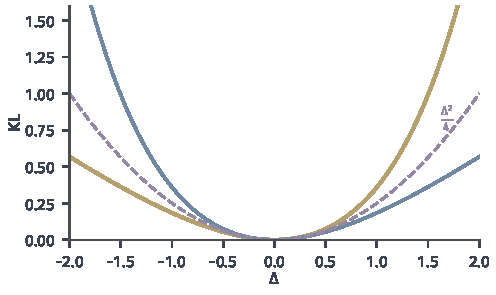
\includegraphics[width=84mm]{figures/07-probability/07-distribution-optimization/matplotlib/igeo-kl-quadratic/figure.pdf}
  \caption{对数方差坐标$\tau=\ln\sigma^{2}$中位移$\Delta$引起的KL散度。蓝线：$D_{\mathrm{KL}}(P_{\tau}\Vert P_{\tau+\Delta})=\frac12(\Delta+\mathrm{e}^{-\Delta}-1)$；黄线：反方向$\frac12(\mathrm{e}^{\Delta}-\Delta-1)$；紫色虚线：二次近似$\frac12G_{\tau\tau}\Delta^{2}=\Delta^{2}/4$。三条曲线在$\Delta=0$附近重合，远处分开。}
  \label{fig:igeo-kl-quadratic}
\end{BookInlineFigure}

局部非退化也推不出全局的参数唯一。在$\mathcal{N}(\theta^{2},1)$中取$\theta=1$，$G(1)=4>0$，二次近似说位移$\delta=-2$应带来约$\frac12\cdot4\cdot4=8$的KL散度；而$\theta+\delta=-1$与$\theta=1$给出同一个分布，真实的KL散度为零。展开只对足够小的$\bm{\delta}$成立，“足够小”有多小，取决于族在这一点附近的形状。

\paragraph{Fisher椭圆}
在二维参数空间中，位移的集合
\[
  \Bigl\{\bm{\delta}:\frac12\bm{\delta}^{\top}\bm{G}(\bm{\theta})\bm{\delta}=\varepsilon\Bigr\}
\]
放在$\bm{\theta}$处是一个以$\bm{\theta}$为中心的椭圆。局部看，椭圆上每个点代表的邻近分布与中心分布的KL散度都约为$\varepsilon$。高斯族在$(\mu,\sigma)$坐标下，由式~\eqref{eq:igeo-gauss-fisher}，椭圆沿$\mu$方向的半轴为$\sigma\sqrt{2\varepsilon}$，沿$\sigma$方向的半轴为$\sigma\sqrt{\varepsilon}$。

图~\ref{fig:igeo-fisher-ellipses}把这些椭圆画在$(\mu,\sigma)$半平面上。同一行的椭圆一样大：平移不改变局部尺度。越靠近$\sigma=0$，椭圆越小：分布越窄，参数只要稍动就造成同样大小的变化。每个椭圆横向比纵向宽$\sqrt2$倍：同样的KL预算下，均值可以比$\sigma$多动一些。把这些椭圆当作各点的“单位圆”，参数平面就带上了一把随位置变化的尺子。

\begin{BookInlineFigure}
  \centering
  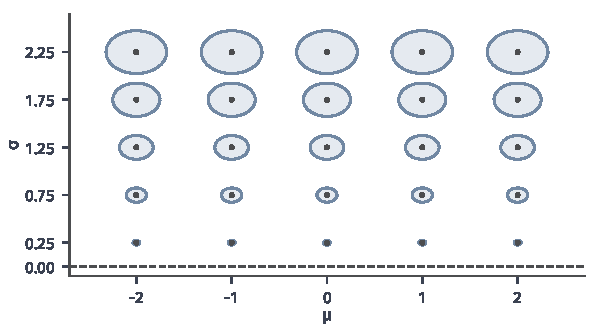
\includegraphics[width=100mm]{figures/07-probability/07-distribution-optimization/matplotlib/igeo-fisher-ellipses/figure.pdf}
  \caption{高斯族在$(\mu,\sigma)$半平面上的Fisher椭圆$\frac12\bm{\delta}^{\top}\bm{G}\bm{\delta}=0.01$。中心为深灰点，$\sigma$取$0.25,0.75,\dots,2.25$，$\mu$取$-2,\dots,2$；半轴为$0.141\sigma$（$\mu$方向）与$0.1\sigma$（$\sigma$方向）。深灰虚线$\sigma=0$不属于参数集合。}
  \label{fig:igeo-fisher-ellipses}
\end{BookInlineFigure}

\subsection{坐标变换}
\label{sec:igeo-coordinates}

同一个高斯族可以用$(\mu,\sigma)$、$(\mu,\sigma^{2})$、$(\mu,\ln\sigma^{2})$或第~\ref{chap:distribution-families}章的自然参数来编号。章首的例子已经显示，同样增加$0.1$，在方差坐标中引起的KL随起点变化，在对数方差坐标中则不变。分布族没有变，变的只是编号的方式。Fisher信息的数值随编号而变，这在章首已经看到；问题是它所表示的“局部变化有多大”是否也依赖于编号。

设$\Xi\subset\mathbb{R}^{k}$是开集，$\bm{\varphi}:\Xi\to\Theta$是连续可微的双射，其逆也连续可微，Jacobian矩阵
\[
  \bm{J}(\bm{\xi})=\frac{\partial\bm{\theta}}{\partial\bm{\xi}}\in\mathbb{R}^{k\times k},\qquad J_{i,j}=\frac{\partial\theta_{i}}{\partial\xi_{j}},
\]
处处非奇异。新坐标下的族是$q_{\bm{\xi}}=p_{\bm{\varphi}(\bm{\xi})}$。它仍是正则族：支撑不变，逐点可微由链式法则得到，而在$\bm{\xi}$的紧邻域上$\bm{J}$有界，原来的控制函数乘以这个界仍然可积。

\begin{theorem}[得分与Fisher信息的坐标变换]
\label{thm:igeo-reparam}
在上述设定下，记$\bm{\theta}=\bm{\varphi}(\bm{\xi})$，$\bm{J}=\bm{J}(\bm{\xi})$，则
\begin{equation}
  \bm{s}^{\Xi}_{\bm{\xi}}(x)=\bm{J}^{\top}\bm{s}_{\bm{\theta}}(x),\qquad
  \bm{G}^{\Xi}(\bm{\xi})=\bm{J}^{\top}\bm{G}(\bm{\theta})\bm{J}.
  \label{eq:igeo-reparam}
\end{equation}
对任意$\mathrm{d}\bm{\xi}\in\mathbb{R}^{k}$，令$\mathrm{d}\bm{\theta}=\bm{J}\,\mathrm{d}\bm{\xi}$，则
\begin{equation}
  \mathrm{d}\bm{\xi}^{\top}\bm{G}^{\Xi}(\bm{\xi})\,\mathrm{d}\bm{\xi}=\mathrm{d}\bm{\theta}^{\top}\bm{G}(\bm{\theta})\,\mathrm{d}\bm{\theta}.
  \label{eq:igeo-invariant-form}
\end{equation}
\end{theorem}

\begin{proof}
由链式法则，对每个$j$，
\[
  \frac{\partial}{\partial\xi_{j}}\ln p_{\bm{\varphi}(\bm{\xi})}(x)=\sum_{i=1}^{k}\frac{\partial\ln p_{\bm{\theta}}(x)}{\partial\theta_{i}}\,\frac{\partial\theta_{i}}{\partial\xi_{j}},
\]
写成向量就是式~\eqref{eq:igeo-reparam}的第一式。$\bm{J}$不随$x$变化，代入式~\eqref{eq:igeo-fisher}，
\[
  \bm{G}^{\Xi}(\bm{\xi})=\mathbb{E}\bigl[\bm{J}^{\top}\bm{s}_{\bm{\theta}}\bm{s}_{\bm{\theta}}^{\top}\bm{J}\bigr]=\bm{J}^{\top}\bm{G}(\bm{\theta})\bm{J}.
\]
最后，
\[
  \mathrm{d}\bm{\xi}^{\top}\bm{J}^{\top}\bm{G}(\bm{\theta})\bm{J}\,\mathrm{d}\bm{\xi}=(\bm{J}\,\mathrm{d}\bm{\xi})^{\top}\bm{G}(\bm{\theta})(\bm{J}\,\mathrm{d}\bm{\xi}),
\]
即式~\eqref{eq:igeo-invariant-form}。
\end{proof}

式~\eqref{eq:igeo-invariant-form}的含义是：$\mathrm{d}\bm{\xi}$与$\mathrm{d}\bm{\theta}=\bm{J}\,\mathrm{d}\bm{\xi}$是同一个无穷小位移在两套坐标中的分量。它们的数字不同，矩阵也不同，但二次型给出同一个值，而由定理~\ref{thm:igeo-kl-expansion}，这个值的一半正是该位移引起的局部KL。改变的是记录方式，不变的是分布本身的局部变化。

\paragraph{方差与对数方差}
在$\mathcal{N}(0,v)$中，$\ln p_{v}(x)=-\frac12\ln(2\pi v)-\frac{x^{2}}{2v}$，于是
\[
  s_{v}(x)=-\frac1{2v}+\frac{x^{2}}{2v^{2}}=\frac{x^{2}-v}{2v^{2}} .
\]
$X^{2}$的方差是$2v^{2}$，所以
\[
  G_{vv}=\frac{\operatorname{Var}(X^{2})}{4v^{4}}=\frac{2v^{2}}{4v^{4}}=\frac1{2v^{2}}.
\]
改用$\tau=\ln v$，$v=\mathrm{e}^{\tau}$，$J=\mathrm{d}v/\mathrm{d}\tau=v$，由式~\eqref{eq:igeo-reparam}，
\[
  G_{\tau\tau}=v^{2}\cdot\frac{1}{2v^{2}}=\frac12 ,
\]
与上一小节由KL展开读出的系数一致。

在$v=4$处取$\Delta v=0.4$，对应$\Delta\tau=\ln1.1\approx0.0953$，一阶近似为$0.1$。两套坐标下的二次型分别是
\[
  \frac12\cdot\frac1{32}\cdot0.4^{2}=0.0025,\qquad\frac12\cdot\frac12\cdot0.1^{2}=0.0025,
\]
完全相等；精确的KL为$0.0022$。而两个位移的欧氏长度一个是$0.4$，一个约是$0.1$。图~\ref{fig:igeo-coordinate-rulers}画出$v=0.5,1,2,4$四处局部KL不超过$0.01$的参数区间：在$v$轴上，区间长度与$v$成正比；在$\tau$轴上，四段一样长。

\begin{BookInlineFigure}
  \centering
  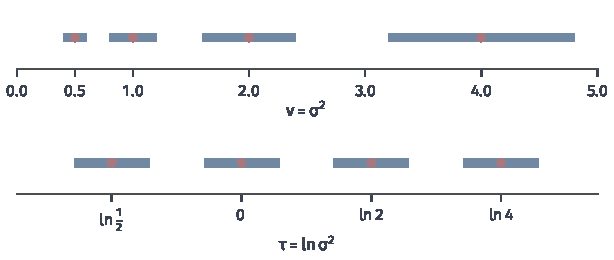
\includegraphics[width=104mm]{figures/07-probability/07-distribution-optimization/matplotlib/igeo-coordinate-rulers/figure.pdf}
  \caption{$\mathcal{N}(0,v)$在$v=0.5,1,2,4$（红点）处满足$\frac12G\,d^{2}\leq0.01$的参数区间（蓝色粗线）。上：方差坐标$v$，半长$0.2v$；下：对数方差坐标$\tau=\ln v$，半长都是$0.2$。两行对应的是同一组分布区间。}
  \label{fig:igeo-coordinate-rulers}
\end{BookInlineFigure}

\paragraph{二维的例子}
把均值加进来。在$(\mu,v)$坐标下，同样的计算给出
\[
  \bm{G}(\mu,v)=\begin{bmatrix}1/v&0\\0&1/(2v^{2})\end{bmatrix},\qquad
  \bm{G}(\mu,\tau)=\begin{bmatrix}1/v&0\\0&1/2\end{bmatrix}.
\]
在$\mathcal{N}(1,4)$处取$(\mu,\tau)$坐标中的位移$(0.6,\ 0.566)$，它满足$\frac12(0.25\cdot0.36+0.5\cdot0.32)=0.125$。换到$(\mu,v)$坐标，$\mathrm{d}v=v\,\mathrm{d}\tau$，位移变为$(0.6,\ 2.263)$，二次型为
\[
  \frac12\Bigl(\frac14\cdot0.36+\frac1{32}\cdot5.12\Bigr)=\frac12(0.09+0.16)=0.125 .
\]
图~\ref{fig:igeo-tangent-ellipses}中，绿色箭头在两张图里的分量相差约四倍，但箭头都恰好落在各自的椭圆$\frac12\bm{\delta}^{\top}\bm{G}\bm{\delta}=0.125$上。

\begin{BookInlineFigure}
  \centering
  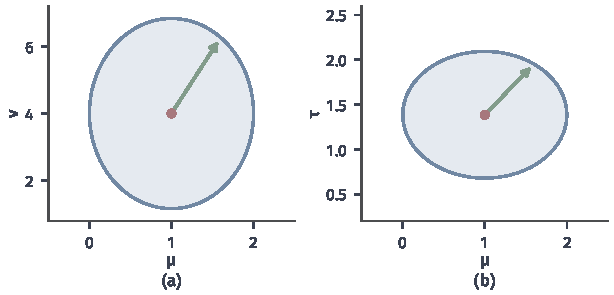
\includegraphics[width=104mm]{figures/07-probability/07-distribution-optimization/matplotlib/igeo-tangent-ellipses/figure.pdf}
  \caption{同一个位移在两套坐标中的表示，中心为$\mathcal{N}(1,4)$（红点）。(a)$(\mu,v)$坐标；(b)$(\mu,\tau)$坐标，$\tau=\ln v$。蓝色椭圆为$\frac12\bm{\delta}^{\top}\bm{G}\bm{\delta}=0.125$，绿色箭头分别是$(0.6,\,2.263)$与$(0.6,\,0.566)$，两者表示同一个位移，都落在椭圆上。两图纵轴的单位不同。}
  \label{fig:igeo-tangent-ellipses}
\end{BookInlineFigure}

\paragraph{几何的说法}
把每一种参数化看成分布族上的一张坐标卡，坐标之间的转换就是流形的坐标变换，无穷小位移就是切向量，它的分量按$\bm{J}$变换，这些概念可参考\BookChapterRef{chap:manifold-basics}{卷四第24章“流形的基本概念”}。式~\eqref{eq:igeo-invariant-form}说明，
\[
  \langle\bm{a},\bm{b}\rangle_{\bm{G}}=\bm{a}^{\top}\bm{G}(\bm{\theta})\bm{b}
\]
是切向量之间不依赖坐标的对称双线性形式。当$\bm{G}$处处正定且光滑变化时，它是参数流形上的一个Riemann度量，称为\term{Fisher度量}（Fisher metric），一般定义可参考\BookChapterRef{chap:riemannian-geometry}{卷四第27章“黎曼几何”}。

这个说法也标出了本节结论的边界。坐标变换下保持的是切向量的长度，即局部变化的大小；矩阵的元素、参数位移的欧氏长度都不保持。在$\bm{G}$退化的点，二次型只是半正定的，不能当作度量，需要先按第~\ref{sec:igeo-fisher}节的办法辨认退化的来源。


\section{指数族的坐标}
\label{sec:igeo-exponential}

前两节的每一步都要单独核验：积分能否与求导交换，得分是否平方可积，Hessian有没有可积的控制。指数族里这些检查都可以一次完成，而且所有的量都由一个函数——对数配分函数——决定。第~\ref{chap:distribution-families}章已经建立了下面的事实：指数族
\[
  p_{\bm{\theta}}(x)=h(x)\exp\bigl(\langle\bm{\theta},\bm{T}(x)\rangle-A(\bm{\theta})\bigr)
\]
相对参考测度$\nu$的所有成员有共同支撑$\{h>0\}$；在自然参数域$\Theta$的内点，$A$无穷次可微，$\bm{T}$的各阶矩有限，并且
\[
  \nabla A(\bm{\theta})=\mathbb{E}_{\bm{\theta}}[\bm{T}],\qquad\nabla^{2}A(\bm{\theta})=\operatorname{Cov}_{\bm{\theta}}(\bm{T}).
\]
在最小表示的正则指数族中，均值映射$\bm{m}=\nabla A$是$\Theta$到开集$\mathcal{M}^{\circ}$的双射，逆映射连续可微。

这一节用这些结论计算得分、Fisher信息与局部KL，并说明自然参数与均值参数两套坐标怎样互相转换。

\paragraph{得分与信息}
在自然参数域的内点，对数密度是$\ln h(x)+\langle\bm{\theta},\bm{T}(x)\rangle-A(\bm{\theta})$，对$\bm{\theta}$求导得到
\begin{equation}
  \bm{s}_{\bm{\theta}}(x)=\bm{T}(x)-\nabla A(\bm{\theta})=\bm{T}(x)-\mathbb{E}_{\bm{\theta}}[\bm{T}].
  \label{eq:igeo-expfam-score}
\end{equation}
得分就是自然统计量减去它的均值，期望为零不需要另外证明。它的协方差就是$\bm{T}$的协方差，于是
\begin{equation}
  \bm{G}(\bm{\theta})=\operatorname{Cov}_{\bm{\theta}}(\bm{T})=\nabla^{2}A(\bm{\theta}).
  \label{eq:igeo-expfam-fisher}
\end{equation}
再求一次导数，对数密度的Hessian是$-\nabla^{2}A(\bm{\theta})$，它不依赖$x$。所以信息等式~\eqref{eq:igeo-information-identity}直接成立；$\nabla^{2}A$连续，在内点的闭球邻域上有界，定理~\ref{thm:igeo-kl-expansion}所需的控制函数可以取常数。正则指数族因此在参数域的每一点都满足前两节的全部条件。

单参数的例子可以从第~\ref{chap:distribution-families}章已算出的导数直接读出。Bernoulli族的自然参数是$\theta=\ln\frac{p}{1-p}$，$G(\theta)=A''(\theta)=p(1-p)$。$\{0,1,2\}$上的倾斜族$p_{\theta}(x)\propto\mathrm{e}^{\theta x}$在$\theta=\ln2$处是$(\frac17,\frac27,\frac47)$，均值为$\frac{10}{7}$，于是
\[
  G(\ln2)=A''(\ln2)=\frac{26}{49}.
\]

高斯族$\mathcal{N}(\mu,\sigma^{2})$取$\bm{T}(x)=(x,x^{2})$，自然参数为$(\mu/\sigma^{2},\,-1/(2\sigma^{2}))$，Fisher信息是$X$与$X^{2}$的协方差矩阵。需要用到高斯分布的三阶与四阶矩：
\[
  \mathbb{E}[X^{3}]=\mu^{3}+3\mu\sigma^{2},\qquad\mathbb{E}[X^{4}]=\mu^{4}+6\mu^{2}\sigma^{2}+3\sigma^{4}.
\]
由此得到
\[
  \operatorname{Cov}(X,X^{2})=\mathbb{E}[X^{3}]-\mu(\mu^{2}+\sigma^{2})=2\mu\sigma^{2},
\]
\[
  \operatorname{Var}(X^{2})=\mathbb{E}[X^{4}]-(\mu^{2}+\sigma^{2})^{2}=4\mu^{2}\sigma^{2}+2\sigma^{4}.
\]
于是自然参数坐标下
\begin{equation}
  \bm{G}(\bm{\theta})=\begin{bmatrix}\sigma^{2}&2\mu\sigma^{2}\\2\mu\sigma^{2}&4\mu^{2}\sigma^{2}+2\sigma^{4}\end{bmatrix}.
  \label{eq:igeo-gauss-natural-fisher}
\end{equation}

例如$\mathcal{N}(1,4)$的自然参数是$(0.25,\,-0.125)$，代入式~\eqref{eq:igeo-gauss-natural-fisher}，信息矩阵为
\[
  \bm{G}=\begin{bmatrix}4&8\\8&48\end{bmatrix}.
\]
它不是对角阵：在自然参数坐标下，两个分量的变化互相纠缠。这个矩阵会在第~\ref{sec:igeo-natural-gradient}节与第~\ref{sec:igeo-implementation}节反复用到。

\paragraph{KL散度是Bregman距离}
在指数族中，KL散度有不必取极限的精确表示。设$\bm{\theta},\bm{\theta}'\in\Theta$都是内点。两个对数密度之差不含$h$：
\[
  \ln\frac{p_{\bm{\theta}}(x)}{p_{\bm{\theta}'}(x)}=\langle\bm{\theta}-\bm{\theta}',\bm{T}(x)\rangle-A(\bm{\theta})+A(\bm{\theta}').
\]
在$P_{\bm{\theta}}$下取期望，$\bm{T}$的期望换成$\nabla A(\bm{\theta})$，得到
\begin{equation}
  D_{\mathrm{KL}}(P_{\bm{\theta}}\Vert P_{\bm{\theta}'})=A(\bm{\theta}')-A(\bm{\theta})-\langle\nabla A(\bm{\theta}),\bm{\theta}'-\bm{\theta}\rangle .
  \label{eq:igeo-expfam-bregman}
\end{equation}

右端是凸函数$A$在$\bm{\theta}'$处的值减去它在$\bm{\theta}$处的切平面的值，称为由$A$生成的\term{Bregman距离}（Bregman distance）。它非负，因为凸函数在切平面之上；它一般不对称，也不满足三角不等式，“距离”只是习惯的叫法。把$A$在$\bm{\theta}$处作二阶Taylor展开，切平面以上的部分是
\[
  \frac12(\bm{\theta}'-\bm{\theta})^{\top}\nabla^{2}A(\bm{\theta})(\bm{\theta}'-\bm{\theta})+o(\lVert\bm{\theta}'-\bm{\theta}\rVert_2^{2}),
\]
由式~\eqref{eq:igeo-expfam-fisher}，这正是定理~\ref{thm:igeo-kl-expansion}在指数族中的形式。

在倾斜族上算一个例子。取$\theta=\ln2$，$\theta'=0$，后者是均匀分布$(\frac13,\frac13,\frac13)$。这个族的对数配分函数是$\ln(1+\mathrm{e}^{\theta}+\mathrm{e}^{2\theta})$，于是$A(0)=\ln3$，$A(\ln2)=\ln7$，代入式~\eqref{eq:igeo-expfam-bregman}，
\[
  D_{\mathrm{KL}}(P_{\ln2}\Vert P_{0})=\ln3-\ln7+\frac{10}{7}\ln2\approx0.1429 .
\]
直接按定义逐项求和，
\[
  \frac17\ln\frac37+\frac27\ln\frac67+\frac47\ln\frac{12}7\approx-0.1210-0.0440+0.3080=0.1430,
\]
在四位小数的舍入范围内一致。二次近似给出$\frac12\cdot\frac{26}{49}\cdot(\ln2)^{2}\approx0.1275$，相差约一成，因为$\ln2\approx0.69$已不算很小的位移。图~\ref{fig:igeo-bregman}(a)中的红色竖线就是这个间隙。

\paragraph{均值坐标}
第~\ref{chap:distribution-families}章说明，在最小表示的正则指数族中，也可以用均值参数$\bm{m}=\mathbb{E}_{\bm{\theta}}[\bm{T}]$给分布编号。均值映射$\bm{m}=\nabla A(\bm{\theta})$的Jacobian矩阵是
\[
  \frac{\partial\bm{m}}{\partial\bm{\theta}}=\nabla^{2}A(\bm{\theta})=\bm{G}(\bm{\theta}),
\]
在最小表示下它正定。由反函数定理（见\BookChapterRef{chap:implicit-inverse-functions}{卷二第22章“隐函数与反函数”}），逆映射$\bm{m}\mapsto\bm{\theta}(\bm{m})$的Jacobian是$\bm{G}(\bm{\theta})^{-1}$。在定理~\ref{thm:igeo-reparam}中取新坐标$\bm{\xi}=\bm{m}$，Jacobian就是$\bm{G}(\bm{\theta})^{-1}$，得到均值坐标下的Fisher信息
\begin{equation}
  \bm{G}^{\mathcal{M}}(\bm{m})=\bm{G}(\bm{\theta})^{-1}\bm{G}(\bm{\theta})\bm{G}(\bm{\theta})^{-1}=\bm{G}(\bm{\theta})^{-1}.
  \label{eq:igeo-mean-fisher}
\end{equation}
同一个Jacobian矩阵既是坐标转换的导数，又是自然坐标中的Fisher信息；而两套坐标中的Fisher信息互为逆矩阵。

Bernoulli族可以直接核对。用$p$作参数，$\ln p_{p}(x)=x\ln p+(1-x)\ln(1-p)$，得分是$\frac{x}{p}-\frac{1-x}{1-p}$，于是
\[
  G^{\mathcal{M}}(p)=p\cdot\frac{1}{p^{2}}+(1-p)\cdot\frac{1}{(1-p)^{2}}=\frac1{p(1-p)},
\]
恰是$G(\theta)=p(1-p)$的倒数。取$\theta=\ln3$，$p=\frac34$，两个值分别是$\frac{3}{16}$与$\frac{16}{3}$。图~\ref{fig:igeo-dual-coordinates}把两条曲线并排画出：自然坐标中，$\lvert\theta\rvert$很大时信息趋于零，一大段参数只对应很小的分布变化；均值坐标中，$p$接近$0$或$1$时信息趋于无穷，$p$稍动，分布的相对变化就很大。两种说法描述的是同一件事。

\begin{BookInlineFigure}
  \centering
  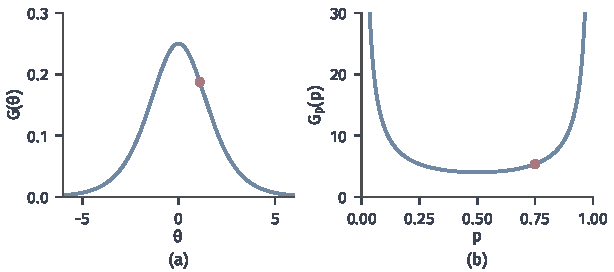
\includegraphics[width=104mm]{figures/07-probability/07-distribution-optimization/matplotlib/igeo-dual-coordinates/figure.pdf}
  \caption{Bernoulli族在两套坐标下的Fisher信息。(a)自然参数$\theta=\ln\frac{p}{1-p}$，$G(\theta)=p(1-p)$；(b)均值参数$p$，$G_{p}(p)=1/(p(1-p))$。红点对应同一个分布$\theta=\ln3$、$p=\frac34$，两值$\frac{3}{16}$与$\frac{16}{3}$互为倒数。}
  \label{fig:igeo-dual-coordinates}
\end{BookInlineFigure}

\paragraph{对偶势函数}
自然坐标有势函数$A$，它的梯度给出均值坐标、Hessian给出Fisher信息。均值坐标也有对应的势函数。在$\mathcal{M}^{\circ}$上令
\begin{equation}
  A^{*}(\bm{m})=\langle\bm{\theta}(\bm{m}),\bm{m}\rangle-A(\bm{\theta}(\bm{m})).
  \label{eq:igeo-dual-potential}
\end{equation}
$A$严格凸，$\bm{\theta}(\bm{m})$是$\langle\bm{\theta},\bm{m}\rangle-A(\bm{\theta})$对$\bm{\theta}$的唯一驻点，因而是最大点，所以
\[
  A^{*}(\bm{m})=\sup_{\bm{\theta}\in\Theta}\bigl\{\langle\bm{\theta},\bm{m}\rangle-A(\bm{\theta})\bigr\},
\]
即$A$的\term{凸共轭}（convex conjugate）在$\mathcal{M}^{\circ}$上的值。它也有概率含义：由式~\eqref{eq:igeo-dual-potential}，$A^{*}(\bm{m})$是$\ln(p_{\bm{\theta}}/h)$在$P_{\bm{\theta}}$下的期望；在有限集上取计数测度且$h=1$时，$A^{*}(\bm{m})$就是$P_{\bm{\theta}}$的负熵$-H(P_{\bm{\theta}})$。

对$\bm{m}$求导，记$\bm{K}=\partial\bm{\theta}/\partial\bm{m}$，
\[
  \nabla A^{*}(\bm{m})=\bm{\theta}+\bm{K}^{\top}\bm{m}-\bm{K}^{\top}\nabla A(\bm{\theta})=\bm{\theta}(\bm{m}),
\]
因为$\nabla A(\bm{\theta})=\bm{m}$，后两项抵消。再求一次导数，
\[
  \nabla^{2}A^{*}(\bm{m})=\frac{\partial\bm{\theta}}{\partial\bm{m}}=\bm{G}(\bm{\theta})^{-1}=\bm{G}^{\mathcal{M}}(\bm{m}).
\]
两个势函数的梯度把两套坐标互相转换，Hessian分别是各自坐标中的Fisher信息，所以这两套坐标常称为一对\term{对偶坐标}（dual coordinates）。

KL散度在均值坐标中也是Bregman距离，只是生成函数换成$A^{*}$，参数的先后次序反过来。由式~\eqref{eq:igeo-dual-potential}，
\[
  A(\bm{\theta})=\langle\bm{\theta},\bm{m}\rangle-A^{*}(\bm{m}),\qquad A(\bm{\theta}')=\langle\bm{\theta}',\bm{m}'\rangle-A^{*}(\bm{m}').
\]
把它们代入式~\eqref{eq:igeo-expfam-bregman}，$\langle\bm{\theta},\bm{m}\rangle$两项抵消，再用$\nabla A^{*}(\bm{m}')=\bm{\theta}'$，得到
\begin{equation}
  D_{\mathrm{KL}}(P_{\bm{\theta}}\Vert P_{\bm{\theta}'})=A^{*}(\bm{m})-A^{*}(\bm{m}')-\langle\nabla A^{*}(\bm{m}'),\bm{m}-\bm{m}'\rangle .
  \label{eq:igeo-dual-bregman}
\end{equation}

在倾斜族的例子中，$m=\frac{10}{7}$，$m'=1$，$(A^{*})'(1)=\theta'=0$，式~\eqref{eq:igeo-dual-bregman}化为
\[
  A^{*}\bigl(\tfrac{10}{7}\bigr)-A^{*}(1)=-H\bigl(\tfrac17,\tfrac27,\tfrac47\bigr)+\ln3\approx0.1429,
\]
与前面的结果相同。图~\ref{fig:igeo-bregman}把两种表示并排画出：同一个KL散度，左边是$A$在$\theta'$处高出切线的量，右边是$A^{*}$在$m$处高出切线的量。

\begin{BookInlineFigure}
  \centering
  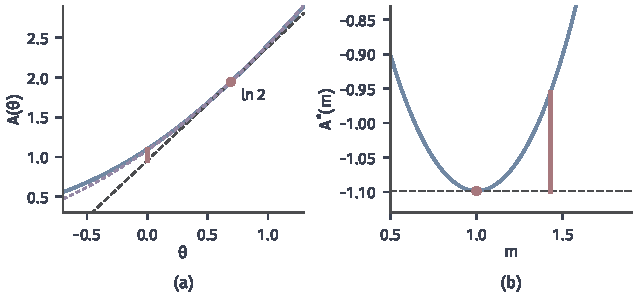
\includegraphics[width=108mm]{figures/07-probability/07-distribution-optimization/matplotlib/igeo-bregman/figure.pdf}
  \caption{$\{0,1,2\}$上倾斜族$p_{\theta}(x)\propto\mathrm{e}^{\theta x}$中$D_{\mathrm{KL}}(P_{\ln2}\Vert P_{0})\approx0.1429$的两种表示（红色竖线）。(a)对数配分函数$A(\theta)$（蓝），深灰虚线为$\theta=\ln2$处的切线（斜率$\frac{10}{7}$），紫色点线为切线加二次项$\frac12\cdot\frac{26}{49}(\theta-\ln2)^{2}$；(b)对偶势函数$A^{*}(m)$（蓝），深灰虚线为$m'=1$处的切线（斜率$0$）。}
  \label{fig:igeo-bregman}
\end{BookInlineFigure}

\paragraph{可逆性失效的情形}
两套坐标的对应依赖两个前提：表示是最小的，参数是自然参数域的内点。去掉任何一个，上面的公式都会出问题。

第一种情形是冗余统计量。Bernoulli族用$x=0$与$x=1$两个示性函数作统计量时，两个分量之和恒为$1$，协方差矩阵
\[
  \bm{G}=\operatorname{Cov}(\bm{T})=p(1-p)\begin{bmatrix}1&-1\\-1&1\end{bmatrix}
\]
处处奇异，零空间沿$(1,1)$方向。沿这个方向改变自然参数，分布不变；均值$(1-p,\,p)$只落在一条直线上，均值映射的像不是$\mathbb{R}^{2}$中的开集，无从定义逆映射。去掉一个统计量回到最小表示，就回到上一段的一维情形。

第二种情形是边界参数。第~\ref{chap:distribution-families}章中$(0,\infty)$上$h(x)=(1+x)^{-2}$、$T(x)=x$的族，参数域是$(-\infty,0]$，边界点$\theta=0$属于参数域，但那里$T$的均值为无穷，得分$T-\mathbb{E}[T]$没有定义，Fisher信息与局部展开都无从谈起。即使边界点不属于参数域，靠近边界时坐标也会失衡：在Bernoulli族中，$\theta\to\pm\infty$时$G(\theta)\to0$，而$p\to0$或$1$时$G^{\mathcal{M}}(p)\to\infty$，族外的点质量$\delta_0$、$\delta_1$不对应任何有限的坐标。


\section{自然梯度}
\label{sec:igeo-natural-gradient}

第~\ref{chap:distribution-approximation}章在参数族$\{Q_{\bm{\theta}}\}$中逼近目标分布$\Pi$，目标函数$L(\bm{\theta})$例如取$D_{\mathrm{KL}}(Q_{\bm{\theta}}\Vert\Pi)$或$D_{\mathrm{KL}}(\Pi\Vert Q_{\bm{\theta}})$。这样的目标是参数的可微函数时，最直接的更新是沿负梯度走一步：$\bm{\theta}\leftarrow\bm{\theta}-\alpha\nabla_{\bm{\theta}}L$。上一节已经看到，参数的同一段欧氏长度在不同位置、不同坐标下代表的分布变化相差悬殊，按欧氏长度分配步伐并没有道理。更合理的问法是：在允许分布发生同样大小的局部变化时，哪个方向使目标下降最多？

本节用一个能手算的例子贯穿。目标分布取$\Pi=\mathcal{N}(0,1)$，候选族为$Q_{\mu,v}=\mathcal{N}(\mu,v)$，目标函数取第~\ref{chap:distribution-approximation}章的$D_{\mathrm{KL}}(Q\Vert\Pi)$。由第~\ref{chap:distribution-comparison}章的高斯KL公式，
\begin{equation}
  L(\mu,v)=-\frac12\ln v+\frac{v+\mu^{2}}{2}-\frac12 .
  \label{eq:igeo-running-objective}
\end{equation}
为了每一步都能核对，这里的目标就在候选族内，最优解$(\mu,v)=(0,1)$是已知的。起点取$\mathcal{N}(1,4)$，那里$L=-\ln2+2\approx1.3069$。

\subsection{受限的下降方向}
\label{sec:igeo-steepest}

记$\bm{g}=\nabla_{\bm{\theta}}L(\bm{\theta})$。参数走一小步$\bm{\delta}$，目标的一阶变化是$\langle\bm{g},\bm{\delta}\rangle$；由定理~\ref{thm:igeo-kl-expansion}，分布的局部变化约为Fisher二次型的一半。给定一个KL预算$\varepsilon>0$，考虑问题
\begin{equation}
  \min_{\bm{\delta}\in\mathbb{R}^{k}}\ \langle\bm{g},\bm{\delta}\rangle\qquad\text{s.t.}\qquad\frac12\bm{\delta}^{\top}\bm{G}(\bm{\theta})\bm{\delta}\leq\varepsilon .
  \label{eq:igeo-steepest-problem}
\end{equation}
若把约束换成$\lVert\bm{\delta}\rVert_2\leq r$，答案是$-\bm{g}$的方向，这就是普通梯度下降。约束换成Fisher二次型以后，答案改变。

\begin{theorem}[Fisher度量下的最速下降方向]
\label{thm:igeo-steepest}
设$\bm{G}=\bm{G}(\bm{\theta})$正定，$\bm{g}\neq\bm{0}$。则问题~\eqref{eq:igeo-steepest-problem}有唯一解
\begin{equation}
  \bm{\delta}^{*}=-\sqrt{\frac{2\varepsilon}{\bm{g}^{\top}\bm{G}^{-1}\bm{g}}}\;\bm{G}^{-1}\bm{g},
  \label{eq:igeo-steepest-solution}
\end{equation}
最小值为
\begin{equation}
  \langle\bm{g},\bm{\delta}^{*}\rangle=-\sqrt{2\varepsilon\,\bm{g}^{\top}\bm{G}^{-1}\bm{g}} .
  \label{eq:igeo-steepest-value}
\end{equation}
\end{theorem}

\begin{proof}
$\bm{G}$正定，所以
\[
  \langle\bm{a},\bm{b}\rangle_{\bm{G}}=\bm{a}^{\top}\bm{G}\bm{b}
\]
是$\mathbb{R}^{k}$上的内积，记相应的范数为$\lVert\cdot\rVert_{\bm{G}}$，约束就是$\bm{\delta}$的这个范数不超过$\sqrt{2\varepsilon}$。把目标的一阶变化写成这个内积：
\[
  \langle\bm{g},\bm{\delta}\rangle=(\bm{G}^{-1}\bm{g})^{\top}\bm{G}\bm{\delta}=\langle\bm{G}^{-1}\bm{g},\bm{\delta}\rangle_{\bm{G}} .
\]
由Cauchy--Schwarz不等式与约束，
\[
  \langle\bm{G}^{-1}\bm{g},\bm{\delta}\rangle_{\bm{G}}\geq-\lVert\bm{G}^{-1}\bm{g}\rVert_{\bm{G}}\,\lVert\bm{\delta}\rVert_{\bm{G}}\geq-\sqrt{\bm{g}^{\top}\bm{G}^{-1}\bm{g}}\,\sqrt{2\varepsilon},
\]
这里用了
\[
  \lVert\bm{G}^{-1}\bm{g}\rVert_{\bm{G}}^{2}=\bm{g}^{\top}\bm{G}^{-1}\bm{G}\bm{G}^{-1}\bm{g}=\bm{g}^{\top}\bm{G}^{-1}\bm{g}.
\]
第一个不等号取等当且仅当$\bm{\delta}=-c\,\bm{G}^{-1}\bm{g}$，$c\geq0$；第二个取等当且仅当$\bm{\delta}$落在椭圆的边界上。两者同时成立唯一确定$c$，即式~\eqref{eq:igeo-steepest-solution}；代入目标，得到式~\eqref{eq:igeo-steepest-value}。
\end{proof}

最优方向与预算$\varepsilon$无关，$\varepsilon$只决定走多远。这个方向值得单独命名。

\begin{definition}[自然梯度]
\label{def:igeo-natural-gradient}
设$\bm{G}(\bm{\theta})$正定。称
\begin{equation}
  \widetilde{\nabla}L(\bm{\theta})=\bm{G}(\bm{\theta})^{-1}\nabla_{\bm{\theta}}L(\bm{\theta})
  \label{eq:igeo-natural-gradient}
\end{equation}
为$L$在$\bm{\theta}$处的\term{自然梯度}（natural gradient）。
\end{definition}

普通梯度相当于假定参数空间各处、各方向的尺度都一样，相当于在一张比例尺处处相同的地图上找最陡的方向。Fisher信息说明这张地图的比例尺因地因向而异：$\bm{G}$大的方向，参数稍动分布就大变，走一小步就要花掉很多预算；$\bm{G}$小的方向，参数要走很远分布才有同样的变化。自然梯度用$\bm{G}^{-1}$把梯度重新分配到这些方向上，便宜的方向多走，贵的方向少走。类比的边界在于，Fisher尺度只在局部成立，它不告诉我们走远以后路面怎样。

\paragraph{例中的两个方向}
在$(\mu,v)$坐标下，由式~\eqref{eq:igeo-running-objective}，
\[
  \bm{g}=\Bigl(\mu,\ \frac12-\frac{1}{2v}\Bigr),\qquad\bm{G}=\begin{bmatrix}1/v&0\\0&1/(2v^{2})\end{bmatrix}.
\]
在起点$(1,4)$处，
\[
  \bm{g}=(1,\ 0.375),\qquad\bm{G}=\operatorname{diag}\bigl(\tfrac14,\ \tfrac1{32}\bigr),\qquad\bm{G}^{-1}\bm{g}=(4,\ 12),
\]
并且$\bm{g}^{\top}\bm{G}^{-1}\bm{g}=4+4.5=8.5$。普通梯度主要指向$\mu$，自然梯度却主要指向$v$：在$v=4$处，$G_{vv}=\frac1{32}$很小，改变方差很“便宜”。

取预算$\varepsilon=0.05$。由式~\eqref{eq:igeo-steepest-solution}，自然梯度步为
\[
  \bm{\delta}_{\mathrm{nat}}=-\sqrt{\frac{0.1}{8.5}}\,(4,\ 12)\approx(-0.434,\ -1.302),
\]
目标的一阶下降为$\sqrt{2\varepsilon\cdot8.5}\approx0.922$。把$-\bm{g}$缩放成$-t\bm{g}$并放到同一个椭圆上，需要
\[
  \frac12t^{2}\,\bm{g}^{\top}\bm{G}\bm{g}=\varepsilon ,
\]
而$\bm{g}^{\top}\bm{G}\bm{g}\approx0.2544$，于是$t\approx0.627$，
\[
  \bm{\delta}_{\mathrm{euc}}=-0.627\,(1,\ 0.375)\approx(-0.627,\ -0.235),
\]
一阶下降为$0.627\times1.1406\approx0.715$。实际代入式~\eqref{eq:igeo-running-objective}，两步之后的目标值分别是$0.513$与$0.789$，起点为$1.307$。

\begin{BookInlineFigure}
  \centering
  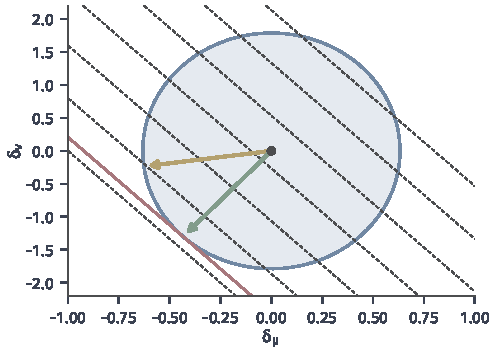
\includegraphics[width=84mm]{figures/07-probability/07-distribution-optimization/matplotlib/igeo-steepest-descent/figure.pdf}
  \caption{$\mathcal{N}(1,4)$处问题~\eqref{eq:igeo-steepest-problem}的几何，坐标为位移$(\delta_{\mu},\delta_{v})$。蓝色椭圆为$\frac12\bm{\delta}^{\top}\bm{G}\bm{\delta}=0.05$，深灰虚线为一阶变化$\langle\bm{g},\bm{\delta}\rangle$的等值线，红线是与椭圆相切的最低等值线。绿色箭头为自然梯度步，黄色箭头为缩放到同一椭圆上的负梯度。}
  \label{fig:igeo-steepest-descent}
\end{BookInlineFigure}

图~\ref{fig:igeo-steepest-descent}把问题~\eqref{eq:igeo-steepest-problem}画了出来。目标的一阶变化在位移平面上是一族平行直线，可行集是Fisher椭圆。最优点是椭圆与最低一条等值线的切点，它在绿色箭头的末端；黄色箭头末端所在的等值线高出不少。这里两个方向的一阶下降比约为$0.78$，差距来自椭圆的扁平程度：在$\bm{G}$各向同性的点，两个方向重合。

把预算想成固定大小的步伐，问题~\eqref{eq:igeo-steepest-problem}就是一种信赖域子问题：在可信的范围内用线性模型选方向，只是范围由分布的变化而不是参数的欧氏距离来划定，可参考\BookChapterRef{chap:trust-region}{卷五第9章“信赖域”}。若$\Pi$本身在候选族内，在最优点$\bm{\theta}^{*}$附近，$D_{\mathrm{KL}}(Q_{\bm{\theta}}\Vert\Pi)$恰好就是$Q_{\bm{\theta}}$与$Q_{\bm{\theta}^{*}}$之间的KL散度，它的Hessian在$\bm{\theta}^{*}$处等于$\bm{G}(\bm{\theta}^{*})$；这时自然梯度在最优点附近与Newton方向几乎一致。

\paragraph{信息矩阵退化时}
定理~\ref{thm:igeo-steepest}要求$\bm{G}$正定。$\bm{G}$奇异时，不能直接写$\bm{G}^{-1}$，而要先回到第~\ref{sec:igeo-fisher}节，辨认退化来自参数冗余还是一阶失效，在有效的坐标上重新建立问题。

先看参数冗余。在$\mathcal{N}(a+b,1)$中逼近$\Pi=\mathcal{N}(1,1)$，记$c=a+b$，目标是$L=\frac12(c-1)^{2}$。梯度与信息矩阵分别是
\[
  \bm{g}=(c-1)\begin{bmatrix}1\\1\end{bmatrix},\qquad\bm{G}=\begin{bmatrix}1&1\\1&1\end{bmatrix}.
\]
$\bm{G}$的零空间沿$(1,-1)$，沿这个方向分布不变，目标也不变，所以$\bm{g}$自动与它正交。去掉冗余，直接用$c$作参数，$G_{cc}=1$，自然梯度是$c-1$。若坚持在$(a,b)$中计算，可以用Moore--Penrose伪逆，$\bm{G}^{\dagger}\bm{g}=\frac{c-1}{2}(1,1)$，它在$c$上引起的变化同样是$c-1$；伪逆只是从无穷多个等价的位移中选了欧氏长度最短的那一个，零空间方向上走多少是任意约定。

再看一阶失效。在$\mathcal{N}(\theta^{3},1)$中逼近同一个$\Pi$，目标是$L=\frac12(\theta^{3}-1)^{2}$，
\[
  g(\theta)=3\theta^{2}(\theta^{3}-1),\qquad G(\theta)=9\theta^{4},\qquad\frac{g(\theta)}{G(\theta)}=\frac{\theta^{3}-1}{3\theta^{2}} .
\]
在$\theta=0$处普通梯度为零，$\theta=0$是$L$的驻点，可分布$\mathcal{N}(0,1)$离最优的$\mathcal{N}(1,1)$还很远；自然梯度则在$\theta\to0$时趋于无穷。两者都是坐标的毛病：用均值$m=\theta^{3}$作参数，$G_{mm}=1$，自然梯度是$m-1$，在$m=0$附近完全正常。

\begin{BookInlineFigure}
  \centering
  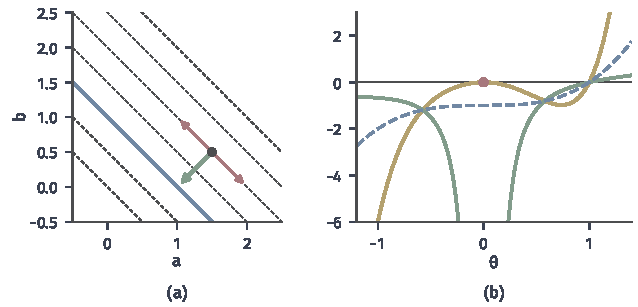
\includegraphics[width=108mm]{figures/07-probability/07-distribution-optimization/matplotlib/igeo-degenerate/figure.pdf}
  \caption{信息矩阵退化的两种情形。(a)$\mathcal{N}(a+b,1)$逼近$\mathcal{N}(1,1)$：深灰虚线是$a+b$为常数的直线，其上分布相同，蓝线$a+b=1$是全部最优参数；在$(1.5,0.5)$处，红色双箭头为$\bm{G}$的零空间方向，绿色箭头为伪逆给出的下降位移。(b)$\mathcal{N}(\theta^{3},1)$逼近$\mathcal{N}(1,1)$：黄线为普通梯度$3\theta^{2}(\theta^{3}-1)$，在红点$\theta=0$处为零；绿线为$g/G=(\theta^{3}-1)/(3\theta^{2})$，在$0$附近发散；蓝色虚线为均值坐标下的自然梯度$m-1$，按$m=\theta^{3}$画在$\theta$轴上。}
  \label{fig:igeo-degenerate}
\end{BookInlineFigure}

图~\ref{fig:igeo-degenerate}对照了这两种情形。实践中常用的另一个办法是把$\bm{G}$换成$\bm{G}+\gamma\bm{I}$，$\gamma>0$，矩阵总是可逆。它能防止数值上的崩溃，却没有回答问题：(b)中$\theta$接近$0$时，加上$\gamma$以后的方向主要由$\gamma$的大小决定，而不是由分布的变化决定。先识别退化方向，再在有效坐标上建立问题，加正则项只作为数值上的保护。

\subsection{重参数化后的更新}
\label{sec:igeo-reparam-update}

普通梯度依赖坐标，这一点从变换公式就能看出。设$\bm{\theta}=\bm{\varphi}(\bm{\xi})$，Jacobian为$\bm{J}$，由链式法则，同一个目标函数在两套坐标中的梯度满足
\[
  \bm{g}_{\bm{\xi}}=\bm{J}^{\top}\bm{g}_{\bm{\theta}} .
\]
在$\bm{\xi}$坐标中沿$-\bm{g}_{\bm{\xi}}$走一小步，换算到$\bm{\theta}$坐标，位移是
\[
  -\bm{J}\bm{g}_{\bm{\xi}}=-\bm{J}\bm{J}^{\top}\bm{g}_{\bm{\theta}} .
\]
除非$\bm{J}\bm{J}^{\top}=\bm{I}$，它与在$\bm{\theta}$坐标中沿$-\bm{g}_{\bm{\theta}}$走的位移不同：两种坐标下的“梯度下降”是两个不同的方向。

自然梯度没有这个问题。由式~\eqref{eq:igeo-reparam}，$\bm{G}^{\Xi}=\bm{J}^{\top}\bm{G}\bm{J}$，于是
\begin{equation}
  \bm{J}\,(\bm{G}^{\Xi})^{-1}\bm{g}_{\bm{\xi}}=\bm{J}\,\bm{J}^{-1}\bm{G}^{-1}\bm{J}^{-\top}\bm{J}^{\top}\bm{g}_{\bm{\theta}}=\bm{G}^{-1}\bm{g}_{\bm{\theta}} .
  \label{eq:igeo-natural-invariance}
\end{equation}
$\bm{\xi}$坐标中的自然梯度换算到$\bm{\theta}$坐标，恰好是$\bm{\theta}$坐标中的自然梯度，两者是同一个切向量。同样，
\[
  \bm{g}_{\bm{\xi}}^{\top}(\bm{G}^{\Xi})^{-1}\bm{g}_{\bm{\xi}}=\bm{g}_{\bm{\theta}}^{\top}\bm{G}^{-1}\bm{g}_{\bm{\theta}},
\]
自然梯度在Fisher度量下的长度也与坐标无关。这与定理~\ref{thm:igeo-steepest}一致：问题~\eqref{eq:igeo-steepest-problem}的目标与约束都只依赖分布，答案自然不依赖于怎样给分布编号。

\paragraph{例中的核对}
把例子改写到自然参数。两套坐标之间的变换是
\[
  (\theta_1,\theta_2)=\Bigl(\frac{\mu}{v},\,-\frac{1}{2v}\Bigr),\qquad(\mu,v)=\Bigl(-\frac{\theta_1}{2\theta_2},\,-\frac{1}{2\theta_2}\Bigr),
\]
起点$\mathcal{N}(1,4)$对应$\bm{\theta}=(0.25,\,-0.125)$。后一个变换的Jacobian在起点处为
\[
  \bm{J}=\frac{\partial(\mu,v)}{\partial(\theta_1,\theta_2)}=\begin{bmatrix}-\frac{1}{2\theta_2}&\frac{\theta_1}{2\theta_2^{2}}\\0&\frac{1}{2\theta_2^{2}}\end{bmatrix}=\begin{bmatrix}4&8\\0&32\end{bmatrix}.
\]
这里$\bm{\theta}$扮演新坐标$\bm{\xi}$的角色。由$\bm{g}_{\bm{\theta}}=\bm{J}^{\top}\bm{g}_{\mu,v}$，
\[
  \bm{g}_{\bm{\theta}}=\begin{bmatrix}4&0\\8&32\end{bmatrix}\begin{bmatrix}1\\0.375\end{bmatrix}=\begin{bmatrix}4\\20\end{bmatrix}.
\]

由式~\eqref{eq:igeo-reparam}算出的信息矩阵是
\[
  \bm{J}^{\top}\begin{bmatrix}\frac14&0\\0&\frac1{32}\end{bmatrix}\bm{J}=\begin{bmatrix}4&8\\8&48\end{bmatrix},
\]
正是第~\ref{sec:igeo-exponential}节由式~\eqref{eq:igeo-gauss-natural-fisher}得到的矩阵。解$\bm{G}\bm{d}=\bm{g}_{\bm{\theta}}$得$\bm{d}=(0.25,\,0.375)$，换算回去，
\[
  \bm{J}\bm{d}=\begin{bmatrix}4\cdot0.25+8\cdot0.375\\32\cdot0.375\end{bmatrix}=\begin{bmatrix}4\\12\end{bmatrix},
\]
正是$(\mu,v)$坐标中的自然梯度，并且$\bm{g}_{\bm{\theta}}^{\top}\bm{d}=1+7.5=8.5$与前面相同。

普通梯度则不然：自然参数中的负梯度$-(4,20)$换算到$(\mu,v)$坐标，是
\[
  -\bm{J}\begin{bmatrix}4\\20\end{bmatrix}=-\begin{bmatrix}176\\640\end{bmatrix},
\]
与$(\mu,v)$坐标中的负梯度$-(1,\ 0.375)$方向不同。

\paragraph{有限步的差别}
自然梯度给出的是切方向，实际更新还要走一个有限步。最简单的规则是在当前坐标中直接相加：$\bm{\theta}\leftarrow\bm{\theta}-\alpha\,\bm{G}^{-1}\bm{g}$。三套坐标下的方向在起点相切，但各自是“直线”的那条曲线并不相同，走出有限距离后到达的分布也不同。

取$\alpha=\frac18$，从$\mathcal{N}(1,4)$出发，在三套坐标中各走一步。在$(\mu,v)$坐标中，自然梯度为$(4,12)$，
\[
  (\mu,v)\leftarrow(1-\tfrac12,\ 4-\tfrac32)=(0.5,\ 2.5).
\]
在自然参数中，自然梯度为$(0.25,0.375)$，
\[
  \bm{\theta}\leftarrow(0.25,\,-0.125)-\tfrac18(0.25,\,0.375)=(0.21875,\,-0.171875),
\]
换回$(\mu,v)\approx(0.636,\ 2.909)$。在$(\mu,\tau)$坐标中，$\tau=\ln v$，信息矩阵为$\operatorname{diag}(1/v,\,\frac12)$，梯度为$(\mu,\ v\,\partial L/\partial v)=(1,\ 1.5)$，自然梯度为$(4,\ 3)$，
\[
  (\mu,\tau)\leftarrow(1-\tfrac12,\ \ln4-\tfrac38),\qquad v=4\mathrm{e}^{-3/8}\approx2.749 .
\]
三个新分布的目标值分别是$0.417$、$0.623$与$0.494$。

另一方面，令步长趋于零，自然梯度更新的连续极限是常微分方程
\begin{equation}
  \dot{\bm{\theta}}(t)=-\bm{G}\bigl(\bm{\theta}(t)\bigr)^{-1}\nabla L\bigl(\bm{\theta}(t)\bigr),
  \label{eq:igeo-natural-flow}
\end{equation}
它的解曲线称为\term{自然梯度流}（natural gradient flow）。由式~\eqref{eq:igeo-natural-invariance}与链式法则，一套坐标中的解换算到另一套坐标，仍满足那里的方程~\eqref{eq:igeo-natural-flow}，所以各坐标给出同一条分布曲线。

在本例的自然参数中，下一节会看到自然梯度恰为$\bm{\theta}-\bm{\theta}_{\Pi}$，其中$\bm{\theta}_{\Pi}=(0,-\frac12)$是目标的自然参数。于是流的解是
\[
  \bm{\theta}(t)=\bm{\theta}_{\Pi}+\mathrm{e}^{-t}\bigl(\bm{\theta}(0)-\bm{\theta}_{\Pi}\bigr).
\]
换到$(\mu,v)$平面，它是线段$v=1+3\mu$。

\begin{BookInlineFigure}
  \centering
  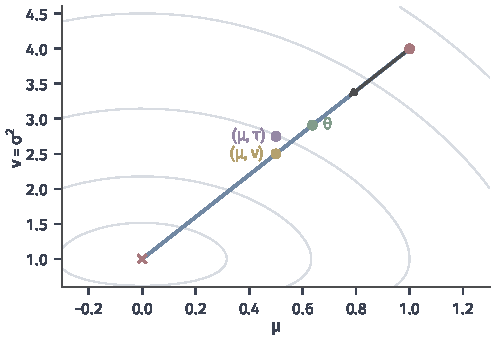
\includegraphics[width=84mm]{figures/07-probability/07-distribution-optimization/matplotlib/igeo-finite-steps/figure.pdf}
  \caption{从$\mathcal{N}(1,4)$（红点）出发、步长$\alpha=\frac18$的一步自然梯度更新，画在$(\mu,v)$平面上，目标为$\mathcal{N}(0,1)$（红叉）。蓝线是自然梯度流，深灰箭头是三套坐标共同的切方向。黄、绿、紫三点分别是在$(\mu,v)$、自然参数$\theta$、$(\mu,\tau)$坐标中直接相加得到的新分布。浅灰线为$L$的等值线。}
  \label{fig:igeo-finite-steps}
\end{BookInlineFigure}

图~\ref{fig:igeo-finite-steps}中，$(\mu,v)$与自然参数两步恰好落在流的直线上，只是走得远近不同；$(\mu,\tau)$一步偏离了这条线。三者一阶相同，二阶以上的差别来自“在坐标中走直线”这一规则本身。若要求有限步也与坐标无关，需要规定从切向量回到参数空间的方式，例如沿Fisher度量的测地线走，或者采用某种满足一阶条件的回缩，这正是流形上的迭代要处理的问题。实际中，这种依赖性通过选择合适的坐标和足够小的步长来控制，并由目标值与参数可行性来检查。


\section{族内更新的实施}
\label{sec:igeo-implementation}

把自然梯度用到第~\ref{chap:distribution-approximation}章的逼近目标上，每一步要做四件事：算出目标的梯度，得到Fisher信息或它与向量的乘积，解一个线性方程得到方向，再定步长并保证新参数仍然合法。前两件常常只能近似完成，后两件则决定了算法在有限步时的表现。

\paragraph{主要思想}
由定义~\ref{def:igeo-natural-gradient}，方向$\bm{d}=\bm{G}^{-1}\bm{g}$。实际计算从不形成逆矩阵，而是解线性方程。为了在$\bm{G}$接近奇异时仍能求解，可以加上一个小的非负数$\gamma$，于是第$t$轮的方向与更新为
\begin{equation}
  \bigl(\bm{G}(\bm{\theta}^{(t)})+\gamma\bm{I}\bigr)\bm{d}^{(t)}=\nabla L(\bm{\theta}^{(t)}),\qquad
  \bm{\theta}^{(t+1)}=\bm{\theta}^{(t)}-\alpha_{t}\,\bm{d}^{(t)}.
  \label{eq:igeo-ngd-update}
\end{equation}
$\gamma=0$时这就是自然梯度步。$\gamma>0$时，$-\bm{d}^{(t)}$是二次模型
\[
  \langle\bm{g},\bm{\delta}\rangle+\frac12\bm{\delta}^{\top}(\bm{G}+\gamma\bm{I})\bm{\delta}
\]
的最小点，相当于在Fisher二次型之外再对参数的欧氏长度加一点惩罚；上一节已经说明，它只是数值上的保护，不能代替对退化方向的分析。

梯度从哪里来，取决于目标的形式。以
\[
  L(\bm{\theta})=D_{\mathrm{KL}}(Q_{\bm{\theta}}\Vert\Pi)=\int q_{\bm{\theta}}\ln\frac{q_{\bm{\theta}}}{\pi}\,\mathrm{d}\nu
\]
为例，$q_{\bm{\theta}}$与$\pi$是相对$\nu$的密度。在积分号下求导需要的条件由第~\ref{chap:expectation-gradient-estimation}章讨论；条件满足时，对被积函数$q_{\bm{\theta}}\ln q_{\bm{\theta}}-q_{\bm{\theta}}\ln\pi$求导，再利用“密度的梯度等于密度乘以得分”与式~\eqref{eq:igeo-score-mean}，得到
\[
  \begin{aligned}
    \nabla L(\bm{\theta})&=\int\nabla q_{\bm{\theta}}\ln\frac{q_{\bm{\theta}}}{\pi}\,\mathrm{d}\nu+\int\nabla q_{\bm{\theta}}\,\mathrm{d}\nu\\
    &=\mathbb{E}_{\bm{\theta}}\Bigl[\bm{s}_{\bm{\theta}}(X)\ln\frac{q_{\bm{\theta}}(X)}{\pi(X)}\Bigr].
  \end{aligned}
\]

在指数族中，由式~\eqref{eq:igeo-expfam-score}，这是$\operatorname{Cov}_{\bm{\theta}}(\bm{T},\ln q_{\bm{\theta}}-\ln\pi)$。若$\Pi$也属于这个族，自然参数为$\bm{\theta}_{\Pi}$，则
\[
  \ln q_{\bm{\theta}}-\ln\pi=\langle\bm{\theta}-\bm{\theta}_{\Pi},\bm{T}\rangle+\text{常数},
\]
于是梯度与自然梯度分别是
\[
  \nabla L(\bm{\theta})=\bm{G}(\bm{\theta})(\bm{\theta}-\bm{\theta}_{\Pi}),\qquad\bm{G}(\bm{\theta})^{-1}\nabla L(\bm{\theta})=\bm{\theta}-\bm{\theta}_{\Pi}.
\]

指数族的自然参数中还有一个省去解方程的办法。目标若写成均值参数的函数，由链式法则与$\partial\bm{m}/\partial\bm{\theta}=\bm{G}$，
\[
  \nabla_{\bm{\theta}}L=\bm{G}(\bm{\theta})\,\nabla_{\bm{m}}L,\qquad\text{从而}\qquad\bm{G}(\bm{\theta})^{-1}\nabla_{\bm{\theta}}L=\nabla_{\bm{m}}L .
\]
在自然参数上走自然梯度步，等于用均值坐标中的普通梯度去更新自然参数。均值坐标下的目标容易求导时，这一形式最省事。

步长分两层控制。第一层是局部预算：由定理~\ref{thm:igeo-steepest}，步长$\alpha$对应的局部KL约为$\frac12\alpha^{2}\,\bm{g}^{\top}\bm{d}$，要它不超过$\varepsilon$，取
\[
  \alpha\leq\sqrt{2\varepsilon/(\bm{g}^{\top}\bm{d})} .
\]
第二层是实际检查：新参数必须属于$\Theta$（例如高斯族的自然参数要求$\theta_2<0$），并且目标要有足够的下降，例如Armijo条件
\begin{equation}
  L(\bm{\theta}-\alpha\bm{d})\leq L(\bm{\theta})-c\,\alpha\,\bm{g}^{\top}\bm{d},\qquad0<c<1 ;
  \label{eq:igeo-armijo}
\end{equation}
不满足就把$\alpha$减半重试，这种回溯可参考\BookChapterRef{chap:smooth-optimization}{卷五第5章“光滑优化基础”}。量$\bm{g}^{\top}\bm{d}$等于$\bm{g}^{\top}\bm{G}^{-1}\bm{g}$，它是自然梯度在Fisher度量下长度的平方，由上一节，它与坐标无关，适合作为停止判据。

\paragraph{计算过程}
下面沿用上一节的例子：目标$\Pi=\mathcal{N}(0,1)$，候选为高斯族，目标函数为式~\eqref{eq:igeo-running-objective}，在自然参数中计算，梯度与信息矩阵都用精确公式。取$\gamma=0$，试探步长$\alpha=\frac12$，Armijo常数$c=10^{-4}$，停止阈值$\mathrm{tol}=10^{-3}$。目标的自然参数是$\bm{\theta}_{\Pi}=(0,\,-0.5)$。

\needspace{6\baselineskip}
\paragraph{变量}
\begin{itemize}
  \item $\bm{\theta}\in\mathbb{R}^{k}$：当前参数，例中$k=2$，并随时换算出$(\mu,v)$。
  \item $\bm{g}\in\mathbb{R}^{k}$：当前梯度$\nabla L(\bm{\theta})$。
  \item $\bm{G}\in\mathbb{R}^{k\times k}$：当前Fisher信息，例中由式~\eqref{eq:igeo-gauss-natural-fisher}计算。
  \item $\bm{C}\in\mathbb{R}^{k\times k}$：$\bm{G}+\gamma\bm{I}$的Cholesky因子，下三角，用后即弃。
  \item $\bm{d}\in\mathbb{R}^{k}$：方向，解方程~\eqref{eq:igeo-ngd-update}得到。
  \item $\alpha$：本轮步长；$L$：当前目标值；$t$：轮次。
\end{itemize}

\paragraph{初始化}
取起点$\bm{\theta}^{(0)}$并检查它属于$\Theta$，算出$L(\bm{\theta}^{(0)})$，令$t=0$。例中起点为$\mathcal{N}(1,4)$，
\[
  \bm{\theta}^{(0)}=(0.25,\ -0.125),\qquad L^{(0)}=-\ln2+2\approx1.3069 .
\]

\needspace{6\baselineskip}
\paragraph{每轮更新}
在第$t$轮：
\begin{enumerate}
  \item \textbf{求梯度与信息矩阵。}计算$\bm{g}=\nabla L(\bm{\theta}^{(t)})$与$\bm{G}=\bm{G}(\bm{\theta}^{(t)})$。例中第一轮$(\mu,v)=(1,4)$，由式~\eqref{eq:igeo-gauss-natural-fisher}与$\bm{g}=\bm{G}(\bm{\theta}-\bm{\theta}_{\Pi})$，
  \[
    \bm{G}=\begin{bmatrix}4&8\\8&48\end{bmatrix},\qquad\bm{g}=\begin{bmatrix}4&8\\8&48\end{bmatrix}\begin{bmatrix}0.25\\0.375\end{bmatrix}=\begin{bmatrix}4\\20\end{bmatrix}.
  \]

  \item \textbf{解方向。}对$\bm{G}+\gamma\bm{I}$作Cholesky分解$\bm{C}\bm{C}^{\top}$，先解$\bm{C}\bm{y}=\bm{g}$，再解$\bm{C}^{\top}\bm{d}=\bm{y}$；分解失败说明矩阵不是正定的，应回到退化分析，而不是继续。例中第一轮
  \[
    \bm{C}=\begin{bmatrix}2&0\\4&4\sqrt2\end{bmatrix}.
  \]
  前代给出
  \[
    y_1=\frac42=2,\qquad y_2=\frac{20-4\cdot2}{4\sqrt2}=\frac{3}{\sqrt2},
  \]
  回代给出
  \[
    d_2=\frac{y_2}{4\sqrt2}=\frac38,\qquad d_1=\frac{2-4\cdot\frac38}{2}=\frac14,
  \]
  即$\bm{d}=(0.25,\,0.375)$。于是$\bm{g}^{\top}\bm{d}=1+7.5=8.5$。

  \item \textbf{检查停止。}若$\bm{g}^{\top}\bm{d}\leq\mathrm{tol}$，输出$\bm{\theta}^{(t)}$并结束。例中第一轮$8.5>10^{-3}$，继续。

  \item \textbf{试探步长。}令$\bm{\theta}'=\bm{\theta}^{(t)}-\alpha\bm{d}$。若$\bm{\theta}'\notin\Theta$，或式~\eqref{eq:igeo-armijo}不成立，把$\alpha$减半重试；成立则接受$\bm{\theta}^{(t+1)}=\bm{\theta}'$，令$t\leftarrow t+1$。例中第一轮
  \[
    \bm{\theta}'=(0.25,\,-0.125)-\tfrac12(0.25,\,0.375)=(0.125,\ -0.3125),
  \]
  $\theta'_2<0$，可行；换算得$v=1/(2\cdot0.3125)=1.6$，$\mu=0.125\cdot1.6=0.2$，由式~\eqref{eq:igeo-running-objective}，
  \[
    L(\bm{\theta}')=-\tfrac12\ln1.6+\tfrac{1.6+0.04}{2}-\tfrac12\approx0.0850 ,
  \]
  远小于Armijo的界$1.3069-10^{-4}\cdot\frac12\cdot8.5$，接受。
\end{enumerate}

例中第二轮从$\mathcal{N}(0.2,\,1.6)$出发。由式~\eqref{eq:igeo-gauss-natural-fisher}，
\[
  \bm{G}=\begin{bmatrix}1.6&0.64\\0.64&5.376\end{bmatrix},\qquad\bm{\theta}-\bm{\theta}_{\Pi}=\begin{bmatrix}0.125\\0.1875\end{bmatrix},\qquad\bm{g}=\begin{bmatrix}0.32\\1.088\end{bmatrix}.
\]
Cholesky因子与解出的方向是
\[
  \bm{C}\approx\begin{bmatrix}1.265&0\\0.506&2.263\end{bmatrix},\qquad\bm{d}=\begin{bmatrix}0.125\\0.1875\end{bmatrix},
\]
其中$C_{2,2}=\sqrt{5.376-0.506^{2}}\approx2.263$。于是
\[
  \bm{g}^{\top}\bm{d}=0.04+0.204=0.244 .
\]
它仍大于阈值。试探步为
\[
  \bm{\theta}'=(0.125,\,-0.3125)-\tfrac12(0.125,\,0.1875)=(0.0625,\ -0.40625),
\]
可行，对应$\mathcal{N}(\frac1{13},\frac{16}{13})$，目标值约$0.0145$，满足式~\eqref{eq:igeo-armijo}，接受。

此后每一轮都重复同样的计算。表~\ref{tab:igeo-ngd-rounds}列出各轮的结果。每轮的$\bm{d}$都等于$\bm{\theta}-\bm{\theta}_{\Pi}$，于是
\[
  \bm{\theta}^{(t)}-\bm{\theta}_{\Pi}=2^{-t}\bigl(\bm{\theta}^{(0)}-\bm{\theta}_{\Pi}\bigr).
\]
第$5$轮开始时$\bm{g}^{\top}\bm{d}\approx3.5\times10^{-4}$，已低于阈值$10^{-3}$，算法停止。最终得到
\[
  \bm{\theta}^{(5)}=\Bigl(\frac1{128},\,-\frac{125}{256}\Bigr),
\]
即$\mathcal{N}(0.008,\,1.024)$，目标值约$1.7\times10^{-4}$。

\begin{BookInlineTable}
  \centering
  \caption{自然梯度迭代的各轮结果，$\alpha=\frac12$，起点$\mathcal{N}(1,4)$，目标$\mathcal{N}(0,1)$。$\bm{g}^{\top}\bm{d}$是本轮开始时自然梯度长度的平方，用于停止判据。}
  \label{tab:igeo-ngd-rounds}
  \begin{tabular}{rrrrr}
    \toprule
    $t$ & $\mu$ & $v$ & $L$ & $\bm{g}^{\top}\bm{d}$ \\
    \midrule
    0 & 1 & 4 & 1.3069 & 8.5 \\
    1 & 0.2 & 1.6 & 0.0850 & 0.244 \\
    2 & 0.0769 & 1.2308 & 0.0145 & 0.0339 \\
    3 & 0.0345 & 1.1034 & 0.00310 & 0.00666 \\
    4 & 0.0164 & 1.0492 & 0.00072 & 0.00149 \\
    5 & 0.0080 & 1.0240 & 0.00017 & 0.00035 \\
    \bottomrule
  \end{tabular}
\end{BookInlineTable}

在这个例子里，若取$\alpha=1$，第一步就直接到达$\bm{\theta}_{\Pi}$。这是因为目标在族内、族是指数族、又在自然参数中计算，三者同时成立时自然梯度恰为$\bm{\theta}-\bm{\theta}_{\Pi}$；一般的逼近问题没有这样的巧合。

\paragraph{算法分析}
先与普通梯度比较。同一个问题在自然参数中用普通梯度，起点处$\bm{g}=(4,20)$，若也取$\alpha=\frac12$，第一步落到$\bm{\theta}=(-1.75,\,-10.125)$，方差约$0.049$，远远越过目标。要避免这种越过，步长要小到约$0.02$；此后在最优点附近，目标的Hessian等于那里的信息矩阵$\operatorname{diag}(1,2)$，每步只把误差缩小约$2\%$。在$(\mu,v)$坐标中用普通梯度、$\alpha=\frac12$，则可以稳定收敛，只是前期较慢。图~\ref{fig:igeo-ngd-runs}对照了三者：普通梯度的表现取决于选哪套坐标，自然梯度的方向则不依赖于这一选择。

\begin{BookInlineFigure}
  \centering
  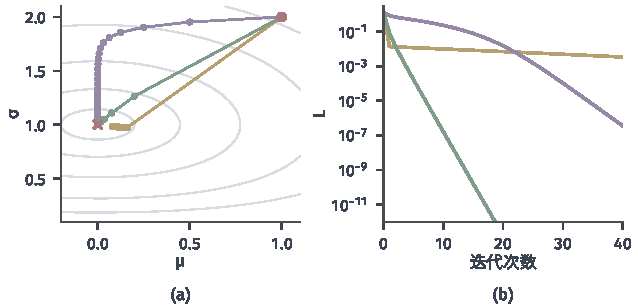
\includegraphics[width=108mm]{figures/07-probability/07-distribution-optimization/matplotlib/igeo-ngd-runs/figure.pdf}
  \caption{从$\mathcal{N}(1,4)$（红点）逼近$\mathcal{N}(0,1)$（红叉），目标$D_{\mathrm{KL}}(Q\Vert\Pi)$，各迭代$40$轮。绿：自然梯度，$\alpha=\frac12$；黄：自然参数中的普通梯度，$\alpha=0.02$；紫：$(\mu,v)$坐标中的普通梯度，$\alpha=\frac12$。(a)迭代点画在$(\mu,\sigma)$平面上，浅灰线为目标的等值线；(b)目标值随迭代次数的变化，纵轴为对数刻度。}
  \label{fig:igeo-ngd-runs}
\end{BookInlineFigure}

收敛方面，表~\ref{tab:igeo-ngd-rounds}的线性收敛是例子的特殊结构给出的。一般情形下，若$L$在非退化的最小点$\bm{\theta}^{*}$附近二阶光滑、$\bm{G}$正定且连续，步长适当时迭代在$\bm{\theta}^{*}$附近线性收敛，速率由$\bm{G}(\bm{\theta}^{*})^{-1}\nabla^{2}L(\bm{\theta}^{*})$的特征值决定；当这个矩阵接近单位阵时，例如目标在族内且用$D_{\mathrm{KL}}(Q\Vert\Pi)$，取$\alpha$接近$1$可以接近Newton法的速度。这只是局部的结论：离最优点很远时，Fisher度量对$L$的曲率没有任何保证，仍要靠回溯和可行性检查。

信息矩阵常常只能估计。由式~\eqref{eq:igeo-fisher}，可以从当前候选分布$Q_{\bm{\theta}}$抽取$n$个独立样本$X_1,\dots,X_n$，用
\begin{equation}
  \widehat{\bm{G}}=\frac1n\sum_{i=1}^{n}\bm{s}_{\bm{\theta}}(X_i)\bm{s}_{\bm{\theta}}(X_i)^{\top}
  \label{eq:igeo-fisher-estimate}
\end{equation}
代替。样本必须来自$Q_{\bm{\theta}}$本身：若改用目标分布的样本计算$\bm{s}_{\bm{\theta}}\bm{s}_{\bm{\theta}}^{\top}$的平均，得到的是得分外积在$\Pi$下的期望，常称为\term{经验Fisher矩阵}（empirical Fisher matrix），除非$Q_{\bm{\theta}}=\Pi$，它不等于$\bm{G}(\bm{\theta})$，所得方向也不再是自然梯度。估计误差按Monte Carlo的速率$n^{-1/2}$缩小，误差分析与方差控制分别见第~\ref{chap:monte-carlo-integration-error}章和第~\ref{chap:variance-reduction}章，梯度本身的随机估计见第~\ref{chap:expectation-gradient-estimation}章。

图~\ref{fig:igeo-fisher-estimate}在例子的起点$\mathcal{N}(1,4)$处做了这一估计。梯度取精确值，$\widehat{\bm{G}}$由$n$个样本得到，方向误差以Fisher范数相对计量。$n=20$时相对误差超过$1$，方向几乎不可信；$n=2000$时约为$8\%$。样本少时，$\widehat{\bm{G}}$的小特征值估计不稳，加上$\gamma$可以避免方向被放大到不合理的长度。

\begin{BookInlineFigure}
  \centering
  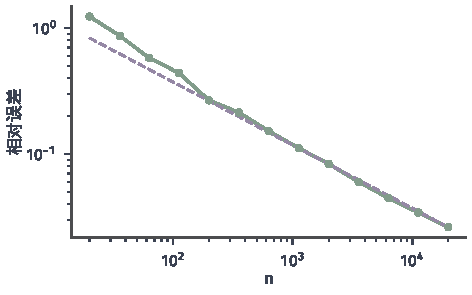
\includegraphics[width=80mm]{figures/07-probability/07-distribution-optimization/matplotlib/igeo-fisher-estimate/figure.pdf}
  \caption{在$\mathcal{N}(1,4)$处用$n$个样本估计自然参数坐标下的Fisher信息，所得方向$\widehat{\bm{d}}=\widehat{\bm{G}}^{-1}\bm{g}$的相对误差$\lVert\widehat{\bm{d}}-\bm{d}\rVert_{\bm{G}}/\lVert\bm{d}\rVert_{\bm{G}}$。绿：$500$次重复的均方根，随机种子$728$；紫色虚线：参考斜率$n^{-1/2}$，在$n=20000$处与绿线对齐。}
  \label{fig:igeo-fisher-estimate}
\end{BookInlineFigure}

计算量方面，用$n$个样本形成$\widehat{\bm{G}}$需要$O(nk^{2})$次运算，Cholesky分解需要$O(k^{3})$，可参考\BookChapterRef{chap:direct-linear-solvers}{卷二第12章“线性方程的直接求解”}。参数维数$k$很大时，两者都负担不起。注意到方程只需要矩阵与向量的乘积，而
\[
  \bm{G}\bm{u}=\mathbb{E}_{\bm{\theta}}\bigl[\bm{s}_{\bm{\theta}}(X)\,\langle\bm{s}_{\bm{\theta}}(X),\bm{u}\rangle\bigr]
\]
可以用同一批样本以$O(nk)$的代价得到，于是可以用共轭梯度法只通过这种\term{Fisher向量积}（Fisher-vector product）近似求解，不必形成$\bm{G}$，可参考\BookChapterRef{chap:krylov-methods}{卷二第15章“Krylov子空间法”}。共轭梯度迭代几步就停止，得到的是近似方向；也可以把$\bm{G}$近似为对角或分块对角矩阵。这些近似都改变了方向，需要用目标值的实际下降来检验。

最后，式~\eqref{eq:igeo-ngd-update}的“在坐标中相加”只是从切向量回到参数空间的一种规则。上一节已经看到，换一套坐标，有限步会到达不同的分布；而参数域的边界，例如方差必须为正，也要单独处理。改用无约束的坐标（如$\tau=\ln v$）、沿测地线移动、或采用满足一阶条件的回缩，都是可选的办法。Fisher度量下的Riemann梯度正是自然梯度，流形上的回缩、向量传输与收敛分析可参考\BookChapterRef{chap:manifold-optimization}{卷五第25章“流形优化”}。

局部几何给出的是方向与尺度，它不代替其他三项检验：迭代是否在全局上收敛，要看目标本身的性质；信息矩阵估计得是否足够准确，要看样本数与方差；族内最优的分布离目标还有多远，是第~\ref{chap:distribution-approximation}章逼近误差的问题，选择更好的更新方向并不能缩小这一差距。


\section{本章小结}
\label{sec:igeo-summary}

章首的问题是：高斯族中同样的参数位移为什么引起大小悬殊的分布变化，这种变化用什么度量，又怎样用于参数更新。本章的回答是一条链：得分描述密度在各处怎样相对变化，Fisher信息把这些变化汇总成参数位移的二次型，邻近分布间的KL散度在二阶意义下正是这个二次型的一半，自然梯度再用这把尺子选取族内更新的方向。图~\ref{fig:igeo-chain-map}标出了链上每一步所需的条件。

\begin{BookInlineFigure}
  \centering
  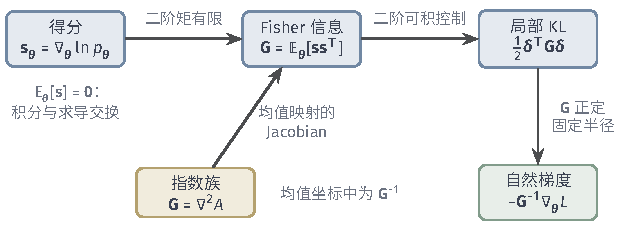
\includegraphics[width=106mm]{figures/07-probability/07-distribution-optimization/tikz/igeo-chain-map/figure.pdf}
  \caption{本章的主线与各步条件。蓝框依次为得分、Fisher信息与局部KL，箭头旁是由前一项得到后一项所需的条件；绿框为自然梯度，需要$\bm{G}$正定；黄框为指数族，其中Fisher信息是对数配分函数的Hessian，也是均值映射的Jacobian。}
  \label{fig:igeo-chain-map}
\end{BookInlineFigure}

正则分布族是这条链的起点：参数集合是开集，支撑不随参数移动，密度对参数可微，并且求导能与积分交换。在这些条件下，得分的期望为零，这是总质量守恒的表现；支撑随参数移动的模型（如$\operatorname{Unif}(0,\theta)$）会多出边界项，KL散度甚至可能为无穷，本章的结论不适用于它们。Fisher信息总是半正定的，但不一定正定。参数冗余、某点的一阶退化与整体不可辨识是三件不同的事，凡要求逆，都要先排除前两种情形。

KL散度的二阶展开说明Fisher信息就是分布变化的局部尺度，系数$\frac12$对应自然对数。它只在一点附近成立：位移稍大，两个方向的KL散度就明显分开，也可能因为整体不可辨识而降到零。换参数坐标时，Fisher信息按$\bm{J}^{\top}\bm{G}\bm{J}$变换，切向量的二次型保持不变。表~\ref{tab:igeo-summary}汇总了高斯族在几套坐标下的结果。

\begin{BookInlineTable}
  \centering
  \caption{高斯族$\mathcal{N}(\mu,\sigma^{2})$在不同坐标下的Fisher信息，$v=\sigma^{2}$，$\tau=\ln v$。各行表示同一个分布族，局部变化的二次型相同。}
  \label{tab:igeo-summary}
  \begin{tabular}{lll}
    \toprule
    坐标 & Fisher信息 & 特点 \\
    \midrule
    $(\mu,\sigma)$ & $\operatorname{diag}(1/\sigma^{2},\,2/\sigma^{2})$ & 尺度随$\sigma$缩小而增大 \\
    $(\mu,v)$ & $\operatorname{diag}(1/v,\,1/(2v^{2}))$ & 方差方向随$v$增大变得便宜 \\
    $(\mu,\tau)$ & $\operatorname{diag}(1/v,\,1/2)$ & 方差方向的尺度处处相同 \\
    自然参数 & $\operatorname{Cov}(X,X^{2})$ & 非对角，等于$\nabla^{2}A$ \\
    均值参数 & 自然参数下信息的逆 & 与自然参数对偶 \\
    \bottomrule
  \end{tabular}
\end{BookInlineTable}

指数族把这些结构集中到对数配分函数上：得分是自然统计量减去均值，Fisher信息是$\nabla^{2}A$，KL散度是由$A$生成的Bregman距离。均值映射的Jacobian就是Fisher信息，所以均值坐标下的Fisher信息是它的逆；对偶势函数$A^{*}$在均值坐标中扮演$A$的角色。这些对应只在最小表示的正则指数族内部成立，冗余统计量与边界参数都会使它失效。

自然梯度是在固定的局部KL预算下使目标一阶下降最多的方向，要求Fisher信息正定、梯度非零。它在坐标变换下表示同一个切向量，普通梯度没有这个性质；但有限步更新还依赖步长和回到参数空间的规则，不同坐标中相加同一个方向，一般得到不同的新分布。实施时，方向由解线性方程得到，信息矩阵可能需要用候选分布自身的样本估计，大规模时只用Fisher向量积近似求解；步长要同时受局部预算、可行性与实际下降的约束。局部几何只回答“朝哪里走、一步走多远才算小”，全局收敛、估计精度与族内逼近误差都需要另外检验。

Fisher信息还出现在统计估计中：它给出由样本估计参数时精度的下界。那是在给定数据下讨论估计量的性质，属于统计推断的问题，可参考\BookChapterRef{chap:finite-sample-lower-bounds}{卷八第5章“有限样本的精度下界”}。

